% !TEX root = ../main.tex
\chapter{一元函数积分学}

学完微分之后，一个自然的问题是：如果知道了一个函数的导数，能不能把原函数找回来？这就是求导的逆运算。

本章先从不定积分入手，逐步引入换元法和分部积分法这两大核心技巧，最后建立定积分与不定积分之间的联系。

\section{不定积分}
微分学告诉我们，对一个函数求导可以得到它的导数。反过来，已知一个函数的导数，求原来的函数，这个逆过程叫做\textbf{求不定积分}。

\subsection{求不定积分}

\begin{definition}{原函数}{}
设函数 $F(x)$ 与 $f(x)$ 都定义在区间 $I$ 上。若对于 $I$ 上每一点 $x$，都有
\[
F'(x) = f(x)
\]
则称 $F(x)$ 是 $f(x)$ 在区间 $I$ 上的一个\textbf{原函数}。
\end{definition}

例如，$F(x)=x^2$ 的导数是 $f(x)=2x$，所以 $x^2$ 是 $2x$ 的一个原函数。但注意，$(x^2+1)'=2x$，$(x^2-5)'=2x$，甚至 $(x^2+C)'=2x$（$C$ 为任意常数）。这说明原函数不是唯一的。因此我们把所有原函数的集合称为不定积分。

\begin{definition}{不定积分}{}
函数 $f(x)$ 在区间 $I$ 上的全体原函数称为 $f(x)$ 的\textbf{不定积分}，记作
\[
\int f(x)\, dx = F(x) + C
\]
其中 $F(x)$ 是 $f(x)$ 的任意一个原函数，$C$ 称为\textbf{积分常数}，$f(x)$ 称为\textbf{被积函数}，$x$ 称为\textbf{积分变量}，符号 $\int$ 称为\textbf{积分号}。
\end{definition}

简单来说，求不定积分，就是找一个函数，使得它的导数等于被积函数，然后在后面加一个常数 $C$。这个 $C$ 绝不能丢，因为导数会抹掉常数信息，积分必须把它补回来。

你可能会问，为什么积分号后面总要拖一个微分 $dx$？那是因为 $dx$ 有几个作用：

首先，$dx$指明积分变量是$x$，$dy$指明积分变量是$y$。例如 $\int x^2 y\, dx$ 和 $\int x^2 y\, dy$ 是完全不同的积分，前者把 $y$ 当常数，对 $x$ 积分，得到 $\frac{x^3}{3}y+C$。后者把 $x^2$ 当常数，对 $y$ 积分，得到 $\frac{x^2 y^2}{2}+C$。意思就是，看到后面的$dx$，就知道是对$x$积分。

让我们先回忆一下微分的定义：$dy = f'(x)\,dx$。把两边同时积分，左边是 $\int dy = y + C$，右边是 $\int f'(x)\,dx=f(x)+C$。也就是说，积分号 $\int$ 和微分号 $d$ 是互逆的运算，$dx$ 正是被积回来的那个微小变化量。

那么$\int f(x)\,dx$ 的意思就是“把 $f(x)$ 和无穷小量 $dx$ 乘起来，得到原函数”。这也是约定俗成的写法。而积分号$\int$正是莱布尼茨发明的。

由于积分是微分的逆运算，我们可以直接把求导公式反过来，得到最基本的积分公式：

\begin{theorem}{基本积分公式}{}
\[
\begin{aligned}
&\text{(1)}\ \int k\, dx = kx + C \quad (k\text{ 为常数})
&&\text{(2)}\ \int x^{\mu}\, dx = \frac{x^{\mu+1}}{\mu+1} + C \quad (\mu \neq -1) \\[4pt]
&\text{(3)}\ \int \frac{1}{x}\, dx = \ln|x| + C
&&\text{(4)}\ \int e^x\, dx = e^x + C \\[4pt]
&\text{(5)}\ \int a^x\, dx = \frac{a^x}{\ln a} + C \quad (a>0,\ a\neq 1)
&&\text{(6)}\ \int \sin x\, dx = -\cos x + C \\[4pt]
&\text{(7)}\ \int \cos x\, dx = \sin x + C
&&\text{(8)}\ \int \sec^2 x\, dx = \tan x + C \\[4pt]
&\text{(9)}\ \int \csc^2 x\, dx = -\cot x + C
&&\text{(10)}\ \int \sec x \tan x\, dx = \sec x + C \\[4pt]
&\text{(11)}\ \int \csc x \cot x\, dx = -\csc x + C
&&\text{(12)}\ \int \frac{1}{1+x^2}\, dx = \arctan x + C \\[4pt]
&\text{(13)}\ \int \frac{1}{\sqrt{1-x^2}}\, dx = \arcsin x + C
\end{aligned}
\]
\end{theorem}

这些公式不需要死记，每一条都可以通过右边求导来验证。

积分还有两条最基本的运算性质，它们直接继承自求导的线性性质：

\begin{theorem}{不定积分的线性性质}{}
设 $f(x)$ 和 $g(x)$ 的原函数都存在，$k$ 为常数，则
\[
\begin{aligned}
&\text{(1)}\quad \int k f(x)\, dx = k \int f(x)\, dx \\[4pt]
&\text{(2)}\quad \int \bigl[f(x) \pm g(x)\bigr]\, dx = \int f(x)\, dx \pm \int g(x)\, dx
\end{aligned}
\]
\end{theorem}

通俗地说，常数因子可以提到积分号外面去，和的积分等于积分的和，差的积分等于积分的差。这两条性质配合基本积分公式，就能处理大多数简单函数的积分了。

\begin{myexample}
  举例说明：求 $ \int (3x^2 + 2x - 1)\, dx$。

  怎么做呢？我们先利用线性性质把被积函数拆成积分的和，也就是：
  $$\int 3x^2 dx + \int 2x dx - \int 1dx$$

  然后把常数提到外面去，也就是：
  $$3\int x^2\, dx + 2\int x\, dx - \int dx$$

  接着，利用基本积分公式，算出每一项的原函数。因为大家都带一个常数，所以可以统一写成一个$C$，也就是：
  $$3 \cdot \frac{x^3}{3} + 2 \cdot \frac{x^2}{2} - x + C$$

  最后化简得到最终结果。

  把过程写出来，就是：
  \[
  \begin{aligned}
  \int (3x^2 + 2x - 1)\, dx
  &= 3\int x^2\, dx + 2\int x\, dx - \int 1\, dx \\
  &= 3 \cdot \frac{x^3}{3} + 2 \cdot \frac{x^2}{2} - x + C \\
  &= x^3 + x^2 - x + C
  \end{aligned}
  \]

\end{myexample}

  我们可以验证一下：

  对结果求导，$(x^3+x^2-x+C)' = 3x^2+2x-1$，与被积函数一致。那就是算对了。

\begin{myexample}
  举例说明：求 $ \int \frac{x^3 - 3x + 2\sqrt{x}}{x}\, dx$。

  先化简被积函数：$\dfrac{x^3 - 3x + 2\sqrt{x}}{x} = x^2 - 3 + 2x^{-\frac{1}{2}}$。

  \[
  \begin{aligned}
  \int (x^2 - 3 + 2x^{-\frac{1}{2}})\, dx
  &= \int x^2\, dx - 3\int 1\, dx + 2\int x^{-\frac{1}{2}}\, dx \\
  &= \frac{x^3}{3} - 3x + 2 \cdot 2\sqrt{x} + C \\
  &= \frac{x^3}{3} - 3x + 4\sqrt{x} + C
  \end{aligned}
  \]
\end{myexample}

这里有一个重要的经验：遇到分式或根式，先化简再积分。很多看起来复杂的积分，化简之后就变成了基本公式的组合。

\begin{myexample}
  举例说明：求 $ \int (\sin x + 2e^x)\, dx$。

  \[
  \int (\sin x + 2e^x)\, dx = \int \sin x\, dx + 2\int e^x\, dx = -\cos x + 2e^x + C
  \]
\end{myexample}

由上述例子可以看出，我们要牢记积分基本公式，才能把积分算出来。

刚刚说到，不定积分和求导互为逆运算，这个关系可以用两句话记住：

先积后导，回到原函数：$ \frac{d}{dx}(\int f(x)\, dx) = f(x)$。

先导后积，回到原函数加常数：$\displaystyle \int F'(x)\, dx = F(x) + C$。

以及，一定一定别忘记加$C$。


\subsection{第一类换元法}

基本积分公式只能处理最简单的被积函数，一旦被积函数是复合函数的形式，比如 $\int \cos 2x \,dx$，基本公式就用不了了。第一类换元法（也叫凑微分法）就是专门解决这类问题的。

第一类换元法直接来源于链式法则的逆用。回忆链式法则：
\[
\frac{d}{dx} F(u(x)) = F'(u(x)) \cdot u'(x) = f(u(x)) \cdot u'(x)
\]

这个式子的意思是对$F(u(x))$求导，等于$F'(u) \cdot u'(x)$，其中 $ F' = f$，$u$是$x$的函数。然后我们两边积分：
\[
\int f(u(x)) \cdot u'(x)\, dx = F(u(x)) + C
\]

因为$u=u(x)$，那么就有$du = u'(x)\, dx$，上式简洁地写成：

\[
\int f(u(x)) \cdot u'(x)\, dx = \int f(u)\, du = F(u) + C
\]

有没有发现有点似曾相识？是的，这正是我们上一章讲到的一阶微分形式不变性。

由此，我们有第一类换元法：
\begin{theorem}{第一类换元法}{}
  设 $F'(u) = f(u)$，且 $u = u(x)$ 可导，则
\[
\int f(u(x)) \cdot u'(x)\, dx = \int f(u)\, du = F(u) + C
\]
\end{theorem}

看上去很复杂，其实就是找一个函数$u(x)$，再把$u'(x)dx$凑出来，然后将被积函数换成关于$u$的函数，$dx$换成$du$，这样整个积分就换成关于$u$的积分，这个积分是要可以用基本公式积出来的，积出来之后再把$x$代回去。

我们来看最开始的例子：

\begin{myexample}
  求 $\int \cos 2x\, dx$。

  令 $u = 2x$，则 $du = 2\, dx$，即 $dx = \frac{1}{2}\, du$。则有：
  \[
  \int \cos 2x\, dx = \int \cos u \cdot \frac{1}{2}\, du
  = \frac{1}{2} \int \cos u\, du
  = \frac{1}{2} \sin u + C
  = \frac{1}{2} \sin 2x + C
  \]
\end{myexample}

仔细看这个例子可以发现，我们令$u = 2x$，由微分公式，$du = 2\, dx$，这时候就能用$du$表示$dx$了。于是整个积分就可以用$u$来表示。这也说明了，凑微分的难点之一在于怎么用我们设的$du$表示$dx$。

再来看一个例子：

\begin{myexample}
  求 $\int 2x \cos x^2\, dx$。

  令 $u = x^2$，则 $du = 2x\, dx$。则有：
  \[
  \int \cos x^2 \cdot 2x\, dx = \int \cos u\, du = \sin u + C = \sin x^2  + C
  \]

\end{myexample}

  这个例子展示了凑微分法的精髓，我们有时候不需要把 $dx$ 单独解出来再代入，而是把 $2x\,dx$ 整体识别为 $du$。我们令$u = x^2$，由微分公式，$du = 2x\, dx$，这时候我们发现被积函数里刚好就有$du = 2x\, dx$，而$\cos x^2$刚好可以表示成$\cos u$，完美。

\begin{myexample}
  求$\int \sin^3 x \cos x\, dx$。

  令$u = \sin x$，则 $du = \cos x\, dx$，则有：

\[
\int \sin^3 x \cdot \cos x\, dx = \int u^3 \, du = \frac{u^4}{4} + C = \frac{\sin^4 x}{4} + C
\]
\end{myexample}

这就是“凑微分”三个字的真正含义，如何在被积表达式里凑出一个完整的 $du$。我们令$u = \sin x$，由微分公式， $du = \cos x\, dx$，这时候我们发现被积函数里刚好就有$du = \cos x\, dx$，和上题类似，直接一套带走。

\begin{myexample}
  求 $\int \frac{1}{2x+1}\, dx$。

  令 $u = 2x+1$，则 $du = 2\, dx$，$dx = \frac{1}{2}\, du$。
  \[
  \int \frac{1}{2x+1}\, dx = \int \frac{1}{u} \cdot \frac{1}{2}\, du
  = \frac{1}{2} \ln|u| + C
  = \frac{1}{2} \ln|2x+1| + C
  \]
\end{myexample}

\begin{myexample}
  求 $\int \tan x\, dx$。

  先把 $\tan x$ 写成 $\frac{\sin x}{\cos x}$。
  
  令 $u = \cos x$，则 $du = -\sin x\, dx$，即 $\sin x\, dx = -du$。
  \[
  \int \tan x\, dx = \int \frac{\sin x}{\cos x}\, dx
  = \int \frac{1}{u} \cdot (-du)
  = -\ln|u| + C
  = -\ln|\cos x| + C
  = \ln|\sec x| + C
  \]

  这个积分非常有用，建议记住它：$\int \tan x\, dx = -\ln|\cos x| + C = \ln|\sec x| + C$。
\end{myexample}

总结一下第一类换元法的核心：

首先通过敏锐的数学直觉，设一个$u=u(x)$，使得被积函数能用$u$来表示，$dx$能用$du$来表示。

然后把原积分换成能用$u$和$du$来表示的基本积分，最后一通操作，直接带走。

以及，一定一定别忘记加$C$。

你可能会说，主播主播这种方法还是太吃技巧了，有没有不吃技巧的方法？有的有的，大部分第一类换元法都围绕这几个形式变形，把他们记住，遇到类似的直接带走就可以了。如果遇到没有的呢？那就借助万能的AI。

\begin{theorem}{线性函数凑微分公式}{}
  含有$ax+b$的积分，可化为以下形式：
\[
\begin{aligned}
&\text{(1)}\ \int (ax+b)^n \,dx = \frac{1}{a}\cdot\frac{(ax+b)^{n+1}}{n+1}+C, \quad n\neq -1 \\[4pt]
&\text{(2)}\ \int \frac{1}{ax+b} \,dx = \frac{1}{a}\ln|ax+b|+C \\[4pt]
&\text{(3)}\ \int e^{ax+b} \,dx = \frac{1}{a}e^{ax+b}+C \\[4pt]
&\text{(4)}\ \int a^{kx+b} \,dx = \frac{1}{k\ln a}a^{kx+b}+C, \quad a>0,a\neq1 \\[4pt]
&\text{(5)}\ \int \sin(ax+b) \,dx = -\frac{1}{a}\cos(ax+b)+C \\[4pt]
&\text{(6)}\ \int \cos(ax+b) \,dx = \frac{1}{a}\sin(ax+b)+C \\[4pt]
&\text{(7)}\ \int \sec^2(ax+b) \,dx = \frac{1}{a}\tan(ax+b)+C \\[4pt]
&\text{(8)}\ \int \csc^2(ax+b) \,dx = -\frac{1}{a}\cot(ax+b)+C \\[4pt]
&\text{(9)}\ \int \sec(ax+b)\tan(ax+b) \,dx = \frac{1}{a}\sec(ax+b)+C \\[4pt]
&\text{(10)}\ \int \csc(ax+b)\cot(ax+b) \,dx = -\frac{1}{a}\csc(ax+b)+C
\end{aligned}
\]
\end{theorem}

我们来看个例子直观感受公式的使用：

\begin{myexample}
  求 $\int ( \frac{4}{2x-1} - \sin(3x-4) + 3e^{5x+2} ) dx$。

  先逐项计算：

令 $u = 2x-1$，则 $du = 2\,dx$，$dx = \frac{1}{2}\,du$。
    \[
    \int \frac{4}{2x-1}\,dx = 4\int \frac{1}{u}\cdot\frac{1}{2}\,du
    = 2\ln|u| + C_1 = 2\ln|2x-1| + C_1
    \]

令 $v = 3x-4$，则 $dv = 3\,dx$，$dx = \frac{1}{3}\,dv$。
    \[
    \int -\sin(3x-4)\,dx = -\int \sin v \cdot \frac{1}{3}\,dv
    = -\frac{1}{3}(-\cos v) + C_2 = \frac{1}{3}\cos(3x-4) + C_2
    \]

令 $w = 5x+2$，则 $dw = 5\,dx$，$dx = \frac{1}{5}\,dw$。
    \[
    \int 3e^{5x+2}\,dx = 3\int e^{w}\cdot\frac{1}{5}\,dw
    = \frac{3}{5}e^{w} + C_3 = \frac{3}{5}e^{5x+2} + C_3
    \]

  相加并合并常数 $C = C_1 + C_2 + C_3$，得：
  \[
  \int ( \frac{4}{2x-1} - \sin(3x-4) + 3e^{5x+2} ) dx
  = 2\ln|2x-1| + \frac{3}{5}e^{5x+2} + \frac{1}{3}\cos(3x-4) + C
  \]

  但是，我们注意到，该积分每一项都是关于线性函数 $ax+b$ 的复合，可直接使用线性函数凑微分公式：

第一项，由公式：$\int \frac{1}{ax+b}\,dx = \frac{1}{a}\ln|ax+b|+C$，其中 $a=2$，$b=-1$，系数 $4$ 提出，得：
    \[
    \int \frac{4}{2x-1}\,dx = 4\cdot\frac{1}{2}\ln|2x-1| + C_1 = 2\ln|2x-1| + C_1
    \]

第二项，由公式：$\int \sin(ax+b)\,dx = -\frac{1}{a}\cos(ax+b)+C$，其中 $a=3$，$b=-4$，注意被积函数有负号，得：
    \[
    \int -\sin(3x-4)\,dx = -(-\frac{1}{3}\cos(3x-4)) + C_2 = \frac{1}{3}\cos(3x-4) + C_2
    \]

第三项，由公式：$\int e^{ax+b}\,dx = \frac{1}{a}e^{ax+b}+C$，其中 $a=5$，$b=2$，得：
    \[
    \int 3e^{5x+2}\,dx = 3\cdot\frac{1}{5}e^{5x+2} + C_3 = \frac{3}{5}e^{5x+2} + C_3
    \]

  相加并合并积分常数 $C = C_1 + C_2 + C_3$，得最终结果：
  \[
  \int ( \frac{4}{2x-1} - \sin(3x-4) + 3e^{5x+2} ) dx
  = 2\ln|2x-1| + \frac{3}{5}e^{5x+2} + \frac{1}{3}\cos(3x-4) + C
  \]
\end{myexample}


\begin{theorem}{幂函数凑微分公式}{}
  含有幂函数的积分，可化为以下形式：
\[
\begin{aligned}
&\text{(1)}\ \int x^n (x^{n+1})^k \,dx = \frac{1}{n+1}\cdot\frac{x^{(n+1)(k+1)}}{k+1}+C, \quad k\neq -1 \\[4pt]
&\text{(2)}\ \int x e^{x^2} \,dx = \frac{1}{2}e^{x^2}+C \\[4pt]
&\text{(3)}\ \int x^n e^{x^{n+1}} \,dx = \frac{1}{n+1}e^{x^{n+1}}+C \\[4pt]
&\text{(4)}\ \int x\sqrt{x^2\pm a^2} \,dx = \frac{1}{3}(x^2\pm a^2)^{\frac{3}{2}}+C \\[4pt]
&\text{(5)}\ \int \frac{x}{\sqrt{x^2\pm a^2}} \,dx = \sqrt{x^2\pm a^2}+C \\[4pt]
&\text{(6)}\ \int x\sin x^2 \,dx = -\frac{1}{2}\cos x^2+C \\[4pt]
&\text{(7)}\ \int x\cos x^2 \,dx = \frac{1}{2}\sin x^2+C \\[4pt]
&\text{(8)}\ \int x\sec^2 x^2 \,dx = \frac{1}{2}\tan x^2+C
\end{aligned}
\]
\end{theorem}

我们再看个例子直观感受公式的使用：

\begin{myexample}
  求 $\int ( 2x e^{x^2} + 3x^2 e^{x^3} - 4x \sin x^2 ) dx$。

    逐项换元计算：

令 $u = x^2$，则 $du = 2x\,dx$，$x\,dx = \frac{1}{2}\,du$。
    \[
    \int 2x e^{x^2}\,dx = \int e^{u}\,du = e^{u} + C_1 = e^{x^2} + C_1
    \]

令 $v = x^3$，则 $dv = 3x^2\,dx$，$x^2\,dx = \frac{1}{3}\,dv$。
    \[
    \int 3x^2 e^{x^3}\,dx = \int e^{v}\,dv = e^{v} + C_2 = e^{x^3} + C_2
    \]

令 $w = x^2$，则 $dw = 2x\,dx$，$x\,dx = \frac{1}{2}\,dw$。
    \[
    \int -4x \sin x^2\,dx = -4\cdot\frac{1}{2}\int \sin w\,dw = -2(-\cos w) + C_3 = 2\cos x^2 + C_3
    \]

  相加并合并常数 $C = C_1+C_2+C_3$，得最终结果：
  \[
  \int ( 2x e^{x^2} + 3x^2 e^{x^3} - 4x \sin x^2 ) dx
  = e^{x^2} + e^{x^3} + 2\cos x^2 + C
  \]

  我们注意到，该积分每一项都是“幂函数乘复合函数”的形式，可直接使用幂函数凑微分公式：

第一项：由公式：$\int x e^{x^2}\,dx = \frac{1}{2}e^{x^2}+C$，系数 $2$ 提出，得：
    \[
    \int 2x e^{x^2}\,dx = 2\cdot\frac{1}{2}e^{x^2}+C_1 = e^{x^2}+C_1
    \]

第二项：由公式：$\int x^n e^{x^{n+1}}\,dx = \frac{1}{n+1}e^{x^{n+1}}+C$，其中$n=2$，系数 $3$ 提出，得：
    \[
    \int 3x^2 e^{x^3}\,dx = 3\cdot\frac{1}{3}e^{x^3}+C_2 = e^{x^3}+C_2
    \]

第三项：由公式：$\int x \sin x^2\,dx = -\frac{1}{2}\cos x^2+C$，系数 $-4$ 提出，得：
    \[
    \int -4x \sin x^2\,dx = -4\cdot(-\frac{1}{2}\cos x^2)+C_3 = 2\cos x^2+C_3
    \]

  相加并合并常数 $C = C_1+C_2+C_3$，得最终结果：
  \[
  \int ( 2x e^{x^2} + 3x^2 e^{x^3} - 4x \sin x^2 ) dx
  = e^{x^2} + e^{x^3} + 2\cos x^2 + C
  \]
\end{myexample}

\begin{theorem}{对数函数凑微分公式}{}
  含有$\ln x$的积分，可化为以下形式：
  \[
\begin{aligned}
&\text{(1)}\ \int \frac{(\ln x)^k}{x} \,dx = \frac{(\ln x)^{k+1}}{k+1}+C, \quad k\neq -1 \\[4pt]
&\text{(2)}\ \int \frac{1}{x\ln x} \,dx = \ln|\ln x|+C \\[4pt]
&\text{(3)}\ \int \frac{1}{x(\ln x)^k} \,dx = \frac{(\ln x)^{1-k}}{1-k}+C, \quad k\neq 1 \\[4pt]
&\text{(4)}\ \int \frac{1}{x\ln x\ln(\ln x)} \,dx = \ln|\ln(\ln x)|+C \\[4pt]
&\text{(5)}\ \int \frac{f'(\ln x)}{x} \,dx = f(\ln x)+C
\end{aligned}
\]
\end{theorem}

\begin{myexample}
  求 $\int ( \frac{(\ln x)^2}{x} + \frac{1}{x\ln x} + \frac{\sin(\ln x)}{x} ) dx$。

  注意到被积函数中反复出现 $\ln x$ 及其导数 $\frac{1}{x}$，可令 $u = \ln x$ 统一换元。

令 $u = \ln x$，则 $du = \frac{1}{x}\,dx$。
    \[
    \int \frac{(\ln x)^2}{x}\,dx = \int u^2\,du = \frac{u^3}{3} + C_1 = \frac{1}{3}(\ln x)^3 + C_1
    \]

同样代换，第二项化为：
    \[
    \int \frac{1}{x\ln x}\,dx = \int \frac{1}{u}\,du = \ln|u| + C_2 = \ln|\ln x| + C_2
    \]

第三项：
    \[
    \int \frac{\sin(\ln x)}{x}\,dx = \int \sin u\,du = -\cos u + C_3 = -\cos(\ln x) + C_3
    \]

  相加并合并常数 $C = C_1+C_2+C_3$，得：
  \[
  \int ( \frac{(\ln x)^2}{x} + \frac{1}{x\ln x} + \frac{\sin(\ln x)}{x} ) dx
  = \frac{1}{3}(\ln x)^3 + \ln|\ln x| - \cos(\ln x) + C
  \]

  也可直接使用对数函数凑微分公式。

第一项：由公式：$\int \frac{(\ln x)^k}{x} \,dx = \frac{(\ln x)^{k+1}}{k+1}+C$，其中 $k=2$，得：
    \[
    \int \frac{(\ln x)^2}{x}\,dx = \frac{(\ln x)^{3}}{3} + C_1
    \]

第二项：由公式：$\int \frac{1}{x\ln x} \,dx = \ln|\ln x|+C$，得：
    \[
    \int \frac{1}{x\ln x}\,dx = \ln|\ln x| + C_2
    \]

第三项：由公式：$\int \frac{f'(\ln x)}{x} \,dx = f(\ln x)+C$，令 $f'(u)=\sin u$，则 $f(u)=-\cos u$，得：
    \[
    \int \frac{\sin(\ln x)}{x}\,dx = -\cos(\ln x) + C_3
    \]

  相加并合并常数 $C = C_1+C_2+C_3$，得：
  \[
  \int ( \frac{(\ln x)^2}{x} + \frac{1}{x\ln x} + \frac{\sin(\ln x)}{x} ) dx
  = \frac{1}{3}(\ln x)^3 + \ln|\ln x| - \cos(\ln x) + C
  \]
\end{myexample}


\begin{theorem}{指数函数凑微分公式}{}
  含有指数函数的积分，可化为以下形式：
  \[
\begin{aligned}
&\text{(1)}\ \int e^{x} f(e^{x}) \,dx = \int f(u)\,du,\; u=e^x \\[4pt]
&\text{(2)}\ \int \frac{e^x}{1+e^{2x}} \,dx = \arctan(e^x)+C \\[4pt]
&\text{(3)}\ \int \frac{e^x}{\sqrt{1-e^{2x}}} \,dx = \arcsin(e^x)+C \\[4pt]
&\text{(4)}\ \int e^{ax}\sin(e^{ax}) \,dx = -\frac{1}{a}\cos(e^{ax})+C \\[4pt]
&\text{(5)}\ \int e^{ax}\cos(e^{ax}) \,dx = \frac{1}{a}\sin(e^{ax})+C \\[4pt]
&\text{(6)}\ \int a^x f(a^x)\,dx = \frac{1}{\ln a}\int f(u)\,du,\; u=a^x \\[4pt]
&\text{(7)}\ \int f'(x)\,e^{f(x)} \,dx = e^{f(x)}+C
\end{aligned}
\]
\end{theorem}

\begin{myexample}
  求 $\int ( \frac{e^{x}}{1+e^{2x}} + 2e^{2x}\sin(e^{2x}) + 2x e^{x^2} ) dx$。

  逐项换元计算：

令 $u = e^{x}$，则 $du = e^{x}\,dx$。
    \[
    \int \frac{e^{x}}{1+e^{2x}}\,dx = \int \frac{1}{1+u^{2}}\,du = \arctan u + C_1 = \arctan(e^{x}) + C_1
    \]

令 $v = e^{2x}$，则 $dv = 2e^{2x}\,dx$，即 $e^{2x}\,dx = \frac{1}{2}\,dv$。
    \[
    \int 2e^{2x}\sin(e^{2x})\,dx = \int \sin v\,dv = -\cos v + C_2 = -\cos(e^{2x}) + C_2
    \]

令 $w = x^{2}$，则 $dw = 2x\,dx$。
    \[
    \int 2x e^{x^{2}}\,dx = \int e^{w}\,dw = e^{w} + C_3 = e^{x^{2}} + C_3
    \]

  相加并合并常数 $C = C_1+C_2+C_3$，得最终结果：
  \[
  \int ( \frac{e^{x}}{1+e^{2x}} + 2e^{2x}\sin(e^{2x}) + 2x e^{x^2} ) dx
  = \arctan(e^x) - \cos(e^{2x}) + e^{x^2} + C
  \]

  也可以直接使用指数函数凑微分公式：

第一项：由公式：$\int \frac{e^x}{1+e^{2x}}\,dx = \arctan(e^x)+C$，得：
    \[
    \int \frac{e^{x}}{1+e^{2x}}\,dx = \arctan(e^x) + C_1
    \]

第二项：由公式：$\int e^{ax}\sin(e^{ax})\,dx = -\frac{1}{a}\cos(e^{ax})+C$，其中 $a=2$，系数 $2$ 提出，得：
    \[
    \int 2e^{2x}\sin(e^{2x})\,dx = 2\cdot(-\frac{1}{2}\cos(e^{2x}))+C_2 = -\cos(e^{2x}) + C_2
    \]

第三项：由公式：$\int f'(x)e^{f(x)}\,dx = e^{f(x)}+C$，令 $f(x)=x^2$，则 $f'(x)=2x$，得：
    \[
    \int 2x e^{x^2}\,dx = e^{x^2} + C_3
    \]

  相加并合并常数 $C = C_1+C_2+C_3$，得最终结果：
  \[
  \int ( \frac{e^{x}}{1+e^{2x}} + 2e^{2x}\sin(e^{2x}) + 2x e^{x^2} ) dx
  = \arctan(e^x) - \cos(e^{2x}) + e^{x^2} + C
  \]
\end{myexample}

\begin{theorem}{三角函数凑微分公式}{}
  含有三角函数的积分，可化为以下形式：
  \[
\begin{aligned}
&\text{(1)}\ \int \tan x \,dx = -\ln|\cos x|+C \\[4pt]
&\text{(2)}\ \int \cot x \,dx = \ln|\sin x|+C \\[4pt]
&\text{(3)}\ \int \sec x \,dx = \ln|\sec x + \tan x|+C \\[4pt]
&\text{(4)}\ \int \csc x \,dx = \ln|\csc x - \cot x|+C \\[4pt]
&\text{(5)}\ \int \tan^n x \sec^2 x \,dx = \frac{\tan^{n+1}x}{n+1}+C, \quad n\neq -1 \\[4pt]
&\text{(6)}\ \int \cot^n x \csc^2 x \,dx = -\frac{\cot^{n+1}x}{n+1}+C, \quad n\neq -1 \\[4pt]
&\text{(7)}\ \int \sin ax \sin bx\,dx = \frac{\sin(a-b)x}{2(a-b)} - \frac{\sin(a+b)x}{2(a+b)} + C,\quad a^2\neq b^2 \\[4pt]
&\text{(8)}\ \int \cos ax \cos bx\,dx = \frac{\sin(a-b)x}{2(a-b)} + \frac{\sin(a+b)x}{2(a+b)} + C,\quad a^2\neq b^2 \\[4pt]
&\text{(9)}\ \int \sin ax \cos bx\,dx = -\frac{\cos(a-b)x}{2(a-b)} - \frac{\cos(a+b)x}{2(a+b)} + C,\quad a^2\neq b^2 \\[4pt]
&\text{(10)}\ \int \sin^{2k+1}x \cos^n x \,dx = -\int (1-\cos^2 x)^k \cos^n x \,d(\cos x) \\[4pt]
&\text{(11)}\ \int \sin^m x \cos^{2k+1}x \,dx = \int \sin^m x (1-\sin^2 x)^k \,d(\sin x) \\[4pt]
&\text{(12)}\ \int \sin^n x\,dx = -\frac{1}{n}\sin^{n-1}x\cos x + \frac{n-1}{n}\int \sin^{n-2}x\,dx \quad (n\ge 2) \\[4pt]
&\text{(13)}\ \int \cos^n x\,dx = \frac{1}{n}\cos^{n-1}x\sin x + \frac{n-1}{n}\int \cos^{n-2}x\,dx \quad (n\ge 2) \\[4pt]
&\text{(14)}\ \int \tan^n x\,dx = \frac{\tan^{n-1}x}{n-1} - \int \tan^{n-2}x\,dx \quad (n\ge 2) \\[4pt]
&\text{(15)}\ \int \cot^n x\,dx = -\frac{\cot^{n-1}x}{n-1} - \int \cot^{n-2}x\,dx \quad (n\ge 2) \\[4pt]
&\text{(16)}\ \int \sec^n x\,dx = \frac{\sec^{n-2}x\tan x}{n-1} + \frac{n-2}{n-1}\int \sec^{n-2}x\,dx \quad (n\ge 2) \\[4pt]
&\text{(17)}\ \int \csc^n x\,dx = -\frac{\csc^{n-2}x\cot x}{n-1} + \frac{n-2}{n-1}\int \csc^{n-2}x\,dx \quad (n\ge 2)
\end{aligned}
\]
\end{theorem}
三角函数没什么好说的，这些都是必背公式。记住就行。


\begin{myexample}
  求 $\int ( 3\sin^{3}(2x-1) + 4\tan^{2}(3x)\sec^{2}(3x) - 2\sec(4x)\tan(4x) ) dx$。

  注意到，每一项都是“线性函数嵌套三角函数”的形式，所以可先对线性函数凑微分，再使用三角函数凑微分公式：

第一项：先线性凑微分，$\int \sin^{3}(2x-1)\,dx = \frac{1}{2}\int \sin^{3}(2x-1)\,d(2x-1)$。
          再由公式：$\int \sin^{n} u\,du = -\frac{1}{n}\sin^{n-1}u\cos u + \frac{n-1}{n}\int \sin^{n-2}u\,du$，其中 $u=2x-1$，$n=3$，系数 $3$ 提出，得：
          \[
          \begin{aligned}
            \int 3\sin^{3}(2x-1)\,dx
            &= \frac{3}{2}\int \sin^{3}u\,du \\
            &= \frac{3}{2}( -\frac{1}{3}\sin^{2}u\cos u + \frac{2}{3}\int \sin u\,du ) \\
            &= \frac{3}{2}( -\frac{1}{3}\sin^{2}u\cos u - \frac{2}{3}\cos u ) + C_{1} \\
            &= \frac{1}{2}\cos^{3}u - \frac{3}{2}\cos u + C_{1} \\
            &= \frac{1}{2}\cos^{3}(2x-1) - \frac{3}{2}\cos(2x-1) + C_{1}
          \end{aligned}
          \]

第二项：线性凑微分 $\int \tan^{2}(3x)\sec^{2}(3x)\,dx = \frac{1}{3}\int \tan^{2}(3x)\sec^{2}(3x)\,d(3x)$。
          由公式：$\int \tan^{n} u \sec^{2} u\,du = \frac{\tan^{n+1}u}{n+1} + C$，其中 $u=3x$，$n=2$，系数 $4$ 提出，得：
          \[
          \int 4\tan^{2}(3x)\sec^{2}(3x)\,dx = 4\cdot\frac{1}{3}\cdot\frac{1}{3}\tan^{3}(3x) + C_{2}
          = \frac{4}{9}\tan^{3}(3x) + C_{2}
          \]

第三项：线性凑微分 $\int \sec(4x)\tan(4x)\,dx = \frac{1}{4}\int \sec(4x)\tan(4x)\,d(4x)$。
          由公式：$\int \sec u \tan u\,du = \sec u + C$，其中 $u=4x$，系数 $-2$ 提出，得：
          \[
          \int -2\sec(4x)\tan(4x)\,dx = -2\cdot\frac{1}{4}\sec(4x) + C_{3} = -\frac{1}{2}\sec(4x) + C_{3}
          \]

合并各项并令 $C = C_{1}+C_{2}+C_{3}$，得最终结果：
\[
\begin{aligned}
\int \bigl( 3\sin^{3}(2x-1) + 4\tan^{2}(3x)\sec^{2}(3x) - 2\sec(4x)\tan(4x) \bigr) dx \\
= \frac{1}{2}\cos^{3}(2x-1) - \frac{3}{2}\cos(2x-1) + \frac{4}{9}\tan^{3}(3x) - \frac{1}{2}\sec(4x) + C
\end{aligned}
\]
\end{myexample}

这说明，实际操作中，往往会有多种函数的复合，这就需要我们火眼金睛，精准地设$u$换元。有时找不出正确的$u$，这是正常现象。只要再多观察一下被积函数，多尝试一下，最后总能发现其中奥秘。如果观察很久之后还是发现不了，那就放弃它，交给AI。

以及，一定一定别忘记加$C$。

最后还有反三角函数。反三角函数出现的机会不多，我们简单带过：


\begin{theorem}{反三角函数凑微分公式}{}
  含有反三角函数的积分，可化为以下形式：
  \[
\begin{aligned}
&\text{(1)}\ \int \frac{1}{\sqrt{a^2-x^2}} \,dx = \arcsin\frac{x}{a}+C, \quad a>0 \\[4pt]
&\text{(2)}\ \int \frac{1}{a^2+x^2} \,dx = \frac{1}{a}\arctan\frac{x}{a}+C \\[4pt]
&\text{(3)}\ \int \frac{1}{x^2-a^2} \,dx = \frac{1}{2a}\ln|\frac{x-a}{x+a}|+C \\[4pt]
&\text{(4)}\ \int \frac{1}{\sqrt{x^2\pm a^2}} \,dx = \ln|x+\sqrt{x^2\pm a^2}|+C \\[4pt]
&\text{(5)}\ \int \frac{1}{x\sqrt{x^2-1}} \,dx = \operatorname{arcsec}|x|+C \\[4pt]
&\text{(6)}\ \int \frac{1}{x\sqrt{1-x^2}} \,dx = -\ln|\frac{1+\sqrt{1-x^2}}{x}|+C \\[4pt]
&\text{(7)}\ \int \frac{\arcsin x}{\sqrt{1-x^2}} \,dx = \frac{1}{2}\arcsin^2 x + C \\[4pt]
&\text{(8)}\ \int \frac{\arctan x}{1+x^2} \,dx = \frac{1}{2}\arctan^2 x + C
\end{aligned}
\]
\end{theorem}

其中，公式$\int \frac{1}{a^2+x^2} \,dx = \frac{1}{a}\arctan\frac{x}{a}+C$和$\int \frac{1}{x^2-a^2} \,dx = \frac{1}{2a}\ln|\frac{x-a}{x+a}|+C$极为重要，应当牢记。

以及，一定一定别忘记加$C$。

\subsection{第二类换元法}

第一类换元法可以看成“从里往外”凑：先设内层函数 $u(x)$，再凑出 $u'(x)\,dx$。但有时候被积函数里有根号，例如 $\int \sqrt{1-x^2}\,dx$，我们根本看不出该凑什么。令 $u = \sqrt{x}$？显然不对。令 $u = 1-x^2$？那 $dx$ 和 $\sqrt{u}$ 搞不到一起去。好像怎么凑都不对。也许你要说，赶紧用AI救一救啊，别急，我们还有一招。

这时候就轮到第二类换元法出场了。第二类换元法可以看成“从外往里”换：我们主动令 $x = \phi(t)$，把整个积分换成关于 $t$ 的形式，希望换完之后根号消失或者变得好处理。由此我们有：

\begin{theorem}{第二类换元法}{}
设 $x = \phi(t)$ 单调可微，且 $\phi'(t) \neq 0$，则
\[
\int f(x)\, dx = \int f(\phi(t)) \cdot \phi'(t)\, dt
\]
\end{theorem}

等我们把右边的积分积出来之后，再把 $x$ 解出来代回去。

有没有发现和第一类换元法很像？第一类换元法是令 $u = u(x)$，然后用$du$表示$dx$。第二类换元法是令 $x = \phi(t)$，然后用$dx$表示 $\phi'(t)\,dt$。方向相反，但本质都是链式法则的逆用。只不过第一类是顺着已有的函数关系凑，第二类是主动创造一个新的函数关系来换。

那么问题来了，令 $x$ 等于什么好呢？第二类换元法最常见的应用场景是被积函数含有 $\sqrt{a^2 - x^2}$、$\sqrt{x^2 + a^2}$、$\sqrt{x^2 - a^2}$ 这三种根式。怎么处理它们呢？不知道你还记不记得，高中数学里有一招叫做三角换元，你还能想起来吗？

想不起来没关系，我们现在带你回忆一下：

\begin{theorem}{三角换元积分公式}{}
\[
\begin{aligned}
&\text{(1)}\ \int \sqrt{a^2 - x^2}\, dx = \frac{a^2}{2}\arcsin\frac{x}{a} + \frac{x}{2}\sqrt{a^2-x^2} + C, \quad a>0 \\[4pt]
&\text{(2)}\ \int \sqrt{x^2 + a^2}\, dx = \frac{x}{2}\sqrt{x^2+a^2} + \frac{a^2}{2}\ln|x + \sqrt{x^2+a^2}| + C \\[4pt]
&\text{(3)}\ \int \sqrt{x^2 - a^2}\, dx = \frac{x}{2}\sqrt{x^2-a^2} - \frac{a^2}{2}\ln|x + \sqrt{x^2-a^2}| + C, \quad a \leq |x|
\end{aligned}
\]
\end{theorem}

我们以第一个公式为例，看看具体的操作：

\begin{myexample}
  求 $\int \sqrt{a^2 - x^2}\, dx$（$a > 0$）。

  看到 $\sqrt{a^2 - x^2}$，怎么处理呢？刚刚说到，用三角换元。怎么换呢？让我们回忆一下，三角换元里利用的是$\sin^2 t + \cos^2 t = 1$，即 $1 - \sin^2 t = \cos^2 t$。那么我们只需要令 $x = a\sin t$，其中 $-\frac{\pi}{2} \leq t \leq \frac{\pi}{2}$，则 $dx = a\cos t\, dt$，$\sqrt{a^2 - x^2} = a\cos t$。根号消失了。

  代入原积分：
  \[
  \int \sqrt{a^2 - x^2}\, dx = \int a\cos t \cdot a\cos t\, dt = a^2 \int \cos^2 t\, dt
  \]

  用半角公式 $\cos^2 t = \frac{1 + \cos 2t}{2}$：
  \[
  a^2 \int \cos^2 t\, dt = a^2\!(\frac{t}{2} + \frac{\sin 2t}{4}) + C = \frac{a^2}{2}t + \frac{a^2}{2}\sin t\cos t + C
  \]

  解出$x$并代回：

  由 $\sin t = \frac{x}{a}$，$\cos t = \frac{\sqrt{a^2-x^2}}{a}$，$t = \arcsin\frac{x}{a}$，得：

  \[
  \int \sqrt{a^2 - x^2}\, dx = \frac{a^2}{2}\arcsin\frac{x}{a} + \frac{x}{2}\sqrt{a^2-x^2} + C
  \]
\end{myexample}

注意代回这一步。令 $x = a\sin t$ 时，$t = \arcsin \frac{x}{a}$，但 $\cos t$ 是多少？硬算的话， $\cos t = \frac{\sqrt{a^2-x^2}}{a}$也可以。不过我们更推荐的是画直角三角形：因为 $\sin t = \frac{x}{a}$，所以我们设角 $t$ 的对边为 $x$、斜边为 $a$，邻边自然就是 $\sqrt{a^2-x^2}$。然后 $\cos t$、$\tan t$ 等都可以直接从这个三角形里读出来，比硬算三角函数快得多。

\begin{center}
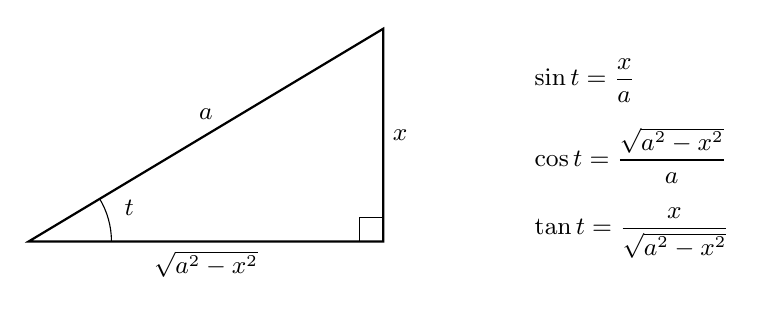
\begin{tikzpicture}[scale=1.5, font=\small]
  % 顶点定义：角 t 在左下 (0,0)，直角在右下 (3,0)，对边顶点在右上 (3,1.8)
  \coordinate (T) at (0,0);   % 锐角 t 的顶点
  \coordinate (R) at (3,0);   % 直角顶点
  \coordinate (P) at (3,1.8); % 对边顶点

  % 三角形
  \draw[thick] (T) -- (R) -- (P) -- cycle;

  % 直角标记（放在 R 处）
  \draw (2.8,0) -- (2.8,0.2) -- (3,0.2);

  % 角 t 的弧线（圆心在 T，从 0° 到 atan(1.8/3)≈31°）
  \draw (0.7,0) arc (0:31:0.7);
  \node at (0.85,0.28) {$t$};

  % 边标注
  \node[below] at (1.5,0) {$\sqrt{a^2-x^2}$};
  \node[right] at (3,0.9) {$x$};
  \node[sloped, above] at (1.5,0.95) {$a$};

  % 右侧公式
  \node[align=left, anchor=west] at (4.2,0.7) {
    \(\displaystyle\sin t = \frac{x}{a}\) \\[8pt]
    \(\displaystyle\cos t = \frac{\sqrt{a^2-x^2}}{a}\) \\[8pt]
    \(\displaystyle\tan t = \frac{x}{\sqrt{a^2-x^2}}\)
  };
\end{tikzpicture}
\end{center}

当然我们不是每次都已知$\sin t = \frac{x}{a}$，可能已知的是其他三角函数值，不过原理是一样的。根据已知三角函数值设边长，求出所有边长之后再算三角函数值即可。后面所有三角换元的代回都可以用这个技巧。

我们再来看第二条公式：

\begin{myexample}
  求 $\int \sqrt{x^2 + a^2}\, dx$（$a > 0$）。

  看到 $\sqrt{x^2 + a^2}$，怎么处理呢？这时候就要用到我们新学的三角恒等式了。因为 $1 + \tan^2 t = \sec^2 t$。设 $x = a\tan t$，其中$-\frac{\pi}{2} < t < \frac{\pi}{2}$，则 $dx = a\sec^2 t\, dt$，$\sqrt{x^2 + a^2} = a\sec t$。根号消失了。

  代入：
  \[
  \int \sqrt{x^2 + a^2}\, dx = \int a\sec t \cdot a\sec^2 t\, dt = a^2 \int \sec^3 t\, dt
  \]

  这里出现了 $\int \sec^3 t\, dt$，由公式：$\int \sec^n t\,dt = \frac{\sec^{n-2}t\tan t}{n-1} + \frac{n-2}{n-1}\int \sec^{n-2}t\,dt$，其中$n=3$，得：
\[
a^2 \int \sec^3 t\,dt =a^2(\frac{\sec t\tan t}{2} + \frac{1}{2}\int \sec t\,dt)
\]

其中 $\int \sec t\,dt$ 由公式：\(\int \sec t\,dt = \ln|\sec t + \tan t| + C\)，得：

\[
a^2 \int \sec^3 t\,dt = a^2 (\frac{1}{2}\sec t \tan t + \frac{1}{2}\ln|\sec t + \tan t|) + C
\]

画三角形：
\begin{center}
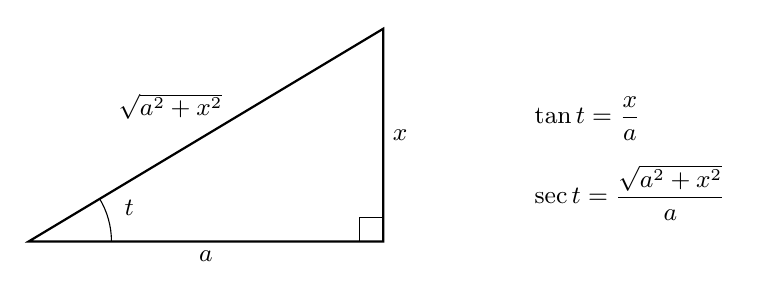
\begin{tikzpicture}[scale=1.5, font=\small]
  % 顶点定义：角 t 在左下 (0,0)，直角在右下 (3,0)，对边顶点在右上 (3,1.8)
  \coordinate (T) at (0,0);   % 锐角 t 的顶点
  \coordinate (R) at (3,0);   % 直角顶点
  \coordinate (P) at (3,1.8); % 对边顶点

  % 三角形
  \draw[thick] (T) -- (R) -- (P) -- cycle;

  % 直角标记（放在 R 处）
  \draw (2.8,0) -- (2.8,0.2) -- (3,0.2);

  % 角 t 的弧线（圆心在 T，从 0° 到 atan(1.8/3)≈31°）
  \draw (0.7,0) arc (0:31:0.7);
  \node at (0.85,0.28) {$t$};

  % 边标注
  \node[below] at (1.5,0) {$a$};
  \node[right] at (3,0.9) {$x$};
  \node[sloped, above] at (1.2,0.95) {$\sqrt{a^2+x^2}$};

  % 右侧公式
  \node[align=left, anchor=west] at (4.2,0.7) {
    \(\displaystyle\tan t = \frac{x}{a}\) \\[8pt]
    \(\displaystyle\sec t = \frac{\sqrt{a^2+x^2}}{a}\)
  };
\end{tikzpicture}
\end{center}

代入原积分，得：
\[
\begin{aligned}
a^2 ( \frac{1}{2}\sec t \tan t + \frac{1}{2}\ln|\sec t + \tan t| ) + C
&= \frac{a^2}{2} \cdot \frac{\sqrt{x^2+a^2}}{a} \cdot \frac{x}{a} + \frac{a^2}{2} \ln| \frac{\sqrt{x^2+a^2}}{a} + \frac{x}{a} | + C \\[4pt]
= \frac{x}{2}\sqrt{x^2+a^2} + \frac{a^2}{2} \ln| \frac{x+\sqrt{x^2+a^2}}{a} | + C 
&= \frac{x}{2}\sqrt{x^2+a^2} + \frac{a^2}{2} \ln| x+\sqrt{x^2+a^2} | - \frac{a^2}{2}\ln a + C
\end{aligned}
\]

将常数 $-\frac{a^2}{2}\ln a$ 并入 $C$，最终得到：
\[
\int \sqrt{x^2+a^2}\,dx = \frac{x}{2}\sqrt{x^2+a^2} + \frac{a^2}{2} \ln| x+\sqrt{x^2+a^2} | + C
\]

\end{myexample}

好了，那么剩下一个$\int \sqrt{x^2 - a^2}\, dx$该怎么做呢？我相信有了前两个例子，聪明的你已经想到怎么做了。不过，实际操作中，我们遇到的往往是它们与其他函数的复合：

\begin{myexample}
  求 $\int \frac{1}{\sqrt{x^2 + 4}}\, dx$。

  设 $x = 2\tan t$，其中 $-\frac{\pi}{2} < t < \frac{\pi}{2}$，则 $dx = 2\sec^2 t\, dt$，$\sqrt{x^2 + 4} = 2\sec t$。

代入：
\[
\int \frac{1}{\sqrt{x^2+4}}\, dx = \int \frac{1}{2\sec t} \cdot 2\sec^2 t\, dt = \int \sec t\, dt
\]

由公式 $\displaystyle \int \sec t\,dt = \ln|\sec t + \tan t| + C$，得：
\[
\int \sec t\,dt = \ln|\sec t + \tan t| + C
\]

画三角形：
\begin{center}
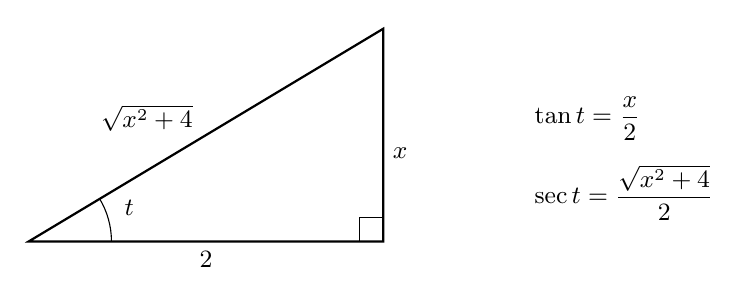
\begin{tikzpicture}[scale=1.5, font=\small]
  % 角 t 在左下 (0,0)，直角在右下 (2,0)，对边顶点在右上 (2,1.5)
  \coordinate (T) at (0,0);   % 锐角 t 的顶点
  \coordinate (R) at (3,0);   % 直角顶点
  \coordinate (P) at (3,1.8); % 对边顶点

  \draw[thick] (T) -- (R) -- (P) -- cycle;

  % 直角标记
  \draw (2.8,0) -- (2.8,0.2) -- (3,0.2);

  % 角 t 弧线
  \draw (0.7,0) arc (0:31:0.7);
  \node at (0.85,0.28) {$t$};

  % 边标注
  \node[below] at (1.5,0) {$2$};
  \node[right] at (3,0.75) {$x$};
  \node[sloped, above] at (1,0.85) {$\sqrt{x^2+4}$};

  % 右侧三角函数值
  \node[align=left, anchor=west] at (4.2,0.7) {
    $\displaystyle\tan t = \frac{x}{2}$ \\[8pt]
    $\displaystyle\sec t = \frac{\sqrt{x^2+4}}{2}$
  };
\end{tikzpicture}
\end{center}

代入原积分，得：
\[
\begin{aligned}
\ln|\sec t + \tan t| + C
&= \ln| \frac{\sqrt{x^2+4}}{2} + \frac{x}{2} | + C \\[4pt]
&= \ln| \frac{x + \sqrt{x^2+4}}{2} | + C \\[4pt]
&= \ln| x + \sqrt{x^2+4} | - \ln 2 + C
\end{aligned}
\]

将常数 $-\ln 2$ 并入 $C$，最终得到：
\[
\int \frac{1}{\sqrt{x^2+4}}\,dx = \ln| x + \sqrt{x^2+4} | + C
\]
\end{myexample}

除了三角换元，还有一种常用的换元是\textbf{根式换元}。当被积函数含有 $\sqrt[n]{ax+b}$ 时，我们令 $t = \sqrt[n]{ax+b}$ 就可以直接把根号消掉。

\begin{theorem}{根式换元积分公式}{}
  \[
\int \sqrt[n]{ax+b}\,dx = \frac{n}{a(n+1)}(ax+b)^{\frac{n+1}{n}} + C \qquad (a\neq 0,\, n\neq -1)
\]
\end{theorem}

背后的原理其实是线性函数凑微分公式：$\int (ax+b)^n \,dx = \frac{1}{a}\cdot\frac{(ax+b)^{n+1}}{n+1}+C$，其中$n\neq -1 $。

\begin{myexample}
  求 $\int \frac{1}{\sqrt{x} + 1}\, dx$。

  被积函数里有 $\sqrt{x}$，我们可以尝试根式换元。令 $t = \sqrt{x}$，则 $x = t^2$，$dx = 2t\, dt$。

  代入原积分：
  \[
  \int \frac{1}{\sqrt{x} + 1}\, dx = \int \frac{1}{t + 1} \cdot 2t\, dt = \int \frac{2t}{t+1}\, dt
  \]

  处理分式：$\frac{2t}{t+1} = 2 - \frac{2}{t+1}$，于是：

  \[
  \int (2 - \frac{2}{t+1}) dt = 2t - 2\ln|t+1| + C = 2\sqrt{x} - 2\ln(\sqrt{x}+1) + C
  \]

\end{myexample}

总结一下第二类换元法的使用场景：

看到 $\sqrt{a^2 - x^2}$，$\sqrt{x^2 + a^2}$，$\sqrt{x^2 - a^2}$，用三角换元。


看到 $\sqrt[n]{ax+b}$，用根式换元。


以及，一定一定别忘记加$C$。


\subsection{分部积分法}

换元法解决的是复合函数型的积分。但还有一类常见的情况：被积函数是两个不同类型函数的乘积，比如 $\int x e^x\,dx$、$\int x \sin x\,dx$。换元法怎么做呢？读者可以先想一想。

想不出来是正常的，因为我们需要另一种工具。

让我们先回忆一下乘法求导法则：
\[
(uv)' = u'v + uv'
\]

两边积分：
\[
\int (uv)'\, dx = \int u'v\, dx + \int uv'\, dx
\]

左边就是 $uv$（省略常数）：
\[
uv = \int u'v\, dx + \int uv'\, dx
\]

移项得：
\[
\int uv'\, dx = uv - \int u'v\, dx
\]

写成微分形式就是：

\begin{theorem}{分部积分公式}{}
\[
\int u\, dv = uv - \int v\, du
\]
\end{theorem}

这个公式的精髓在于，右边的 $\int v\, du$ 可能比左边的 $\int u\, dv$ 更好积分。关键在于怎么选 $u$ 和 $dv$。选对了，直接一通带走。选错了，可能越积越复杂。

一般的经验法则是\textbf{把容易求导的函数选为 $u$，把容易积分的函数选为 $dv$}。一般来说，按“对、反、幂、三、指”的优先级选择 $u$，也就是：
\begin{center}
  对数函数$>$反三角函数$>$幂函数$>$三角函数$>$指数函数
\end{center}



来看几个例子。

\begin{myexample}
  求 $\int x e^x\, dx$。

  分析被积函数，这是一个幂函数和一个指数函数相乘。根据“对数函数$>$反三角函数$>$幂函数$>$三角函数$>$指数函数”，那么我们应该选$x$作为$u$。

  令 $u = x$，$dv = e^x\, dx$。则 $du = dx$，$v = e^x$。
  
  代入公式：
  \[
  \int x e^x\, dx = x e^x - \int e^x\, dx = x e^x - e^x + C = (x-1)e^x + C
  \]

\end{myexample}

我们可以验证一下：$((x-1)e^x + C)' = e^x + (x-1)e^x = x e^x$，没问题。

这个例子展示了分部积分法的核心思想：$x$ 求导后变成 $1$，$e^x$ 积分后还是 $e^x$，所以右边的 $\int e^x\,dx$ 变得非常简单。

\begin{myexample}
  求 $\int x \sin x\, dx$。

  分析被积函数，这是一个幂函数和一个三角函数相乘。根据“对数函数$>$反三角函数$>$幂函数$>$三角函数$>$指数函数”，那么我们应该选$x$作为$u$。

  令 $u = x$，$dv = \sin x\, dx$。则 $du = dx$，$v = -\cos x$。
  
  代入公式：
  \[
  \int x \sin x\, dx = -x\cos x - \int (-\cos x)\, dx = -x\cos x + \int \cos x\, dx = -x\cos x + \sin x + C
  \]
\end{myexample}

\begin{myexample}
  求 $\int \ln x\, dx$。

  这个积分没有乘积怎么办？其实，这个积分可以看成 $\int 1 \cdot \ln x\, dx$。分析被积函数，这是一个常数函数和一个对数函数相乘。根据“对数函数$>$反三角函数$>$幂函数$>$三角函数$>$指数函数”，那么我们应该选$\ln x$作为$u$。
  
  令 $u = \ln x$，$dv = dx$。则 $du = \frac{1}{x}\, dx$，$v = x$。
  
  代入公式：
  \[
  \int \ln x\, dx = x\ln x - \int x \cdot \frac{1}{x}\, dx = x\ln x - \int 1\, dx = x\ln x - x + C
  \]

\end{myexample}

  这个结果非常有用，建议记住：$\int \ln x\, dx = x\ln x - x + C$。
  
  有些积分需要连续使用两次分部积分，比如：

\begin{myexample}
  求 $\int e^x \sin x\, dx$。

  分析被积函数，这是一个指数函数和一个三角函数相乘。根据“对数函数$>$反三角函数$>$幂函数$>$三角函数$>$指数函数”，那么我们应该选$\sin x$作为$u$。

  令 $u = \sin x$，$dv = e^x\, dx$。则 $du = \cos x\, dx$，$v = e^x$。

  代入公式：
  \[
  \int e^x \sin x\, dx = e^x \sin x - \int e^x \cos x\, dx
  \]

  右边出现了 $\int e^x \cos x\, dx$，这时候我们可以再用一次分部积分。
  
  令 $u = \cos x$，$dv = e^x\, dx$，则 $du = -\sin x\, dx$，$v = e^x$。
  
  代入公式：
  \[
  \int e^x \cos x\, dx = e^x \cos x - \int e^x (-\sin x)\, dx = e^x \cos x + \int e^x \sin x\, dx
  \]

  代入原积分：
  \[
  \int e^x \sin x\, dx = e^x \sin x - (e^x \cos x + \int e^x \sin x\, dx)
  \]

  这时候我们发现，右边又出现了 $\int e^x \sin x\, dx$，我们把它移到左边：
  \[
  2\int e^x \sin x\, dx = e^x \sin x - e^x \cos x + C
  \]

  两边除以 $2$：
  \[
  \int e^x \sin x\, dx = \frac{e^x(\sin x - \cos x)}{2} + C
  \]
\end{myexample}

这个例子展示了分部积分的一个神奇现象，当某些积分连续用了两次分部积分法的时候，原来的积分“绕回来了”。这时候把它当成一个未知数，解方程就能得到结果。这种技巧叫做“循环分部积分”，遇到 $e^x$ 和三角函数的乘积时经常用到。

总结一下分部积分法的核心，就是选择关键的$u$和$dv$，大部分时候分部积分都是两个函数的乘积，按照优先级选择$u$基本不会选错。

以及，一定一定别忘记加$C$。

虽然说我们用上述方法能解出大部分的不定积分，但是有些积分是我们很难解或者不能用初等函数表示的。

例如我们口算都能算出来\(\int \frac{1}{x^5} dx=-\frac{1}{4x^4}+C\)，但是\(\int \frac{1}{1+x^5}dx\)等于多少呢？

实际上，这是一个非常难算的积分：

\[
\begin{aligned}
\int \frac{dx}{1+x^5} 
&= \frac{1}{5}\ln|x+1| 
- \frac{1}{20}\ln\!(x^4 - x^3 + x^2 - x + 1) \\[4pt]
&\quad + \frac{1}{5}\sqrt{\frac{5+\sqrt{5}}{2}}\;
\arctan\!(\frac{4x - 1 + \sqrt{5}}{\sqrt{10 - 2\sqrt{5}}}) \\[4pt]
&\quad + \frac{1}{5}\sqrt{\frac{5-\sqrt{5}}{2}}\;
\arctan\!(\frac{4x - 1 - \sqrt{5}}{\sqrt{10 + 2\sqrt{5}}}) + C
\end{aligned}
\]

更进一步的，\(\int \frac{1}{1+x+x^5}dx\)等于多少呢？

还有一些积分根本无法用初等函数表达。例如：

\[
\begin{aligned}
&\int e^{-x^2}\,dx,\qquad \int \sin x^2\,dx,\qquad \int \cos x^2\,dx,\qquad \int \frac{\sin x}{x}\,dx,\qquad \int \frac{\cos x}{x}\,dx,\\
&\int \frac{e^x}{x}\,dx,\qquad \int \frac{1}{\ln x}\,dx,\qquad \int \frac{dx}{\sqrt{1-k^2\sin^2 x}},\qquad \int \sqrt{1-k^2\sin^2 x}\,dx,\\
&\int \frac{dx}{\sqrt{x^3+1}},\qquad \int \ln \ln x\,dx,\qquad \int \sin\!(\frac{1}{x})dx,\qquad \int x^x\,dx
\end{aligned}
\]

不相信？自己动手算算呗。

\section{定积分}
我们已经学会了导数，学会了不定积分。现在我们要把无数个瞬间的微小结果重新累积起来，求得一个确定的总量，这就是定积分。至此，我们算是踏进了微积分的大门。

\subsection{定积分的几何意义}

想象一下，你在平面上画了一条曲线 $y = f(x)$（假设 $f(x) \geq 0$），然后在 $x$ 轴上标出区间 $[a, b]$。这条曲线、$x$ 轴以及两条竖直线 $x = a$ 和 $x = b$ 围成的区域，就是所谓的\textbf{曲边梯形}。定积分 $\int_a^b f(x)\,dx$ 的几何意义就是这个曲边梯形的面积。

\begin{center}
  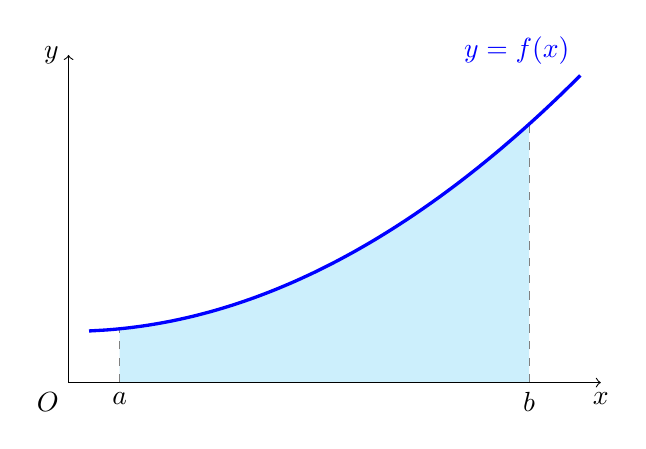
\begin{tikzpicture}[scale=1.3]
    % 定义函数和区间
    \def\a{0.5}     % 左端点
    \def\b{4.5}     % 右端点
    
    % 先填充曲边梯形区域（曲线下方，从 a 到 b）
    \fill[cyan!20] 
        plot[domain=\a:\b, smooth] (\x, {0.1*\x*\x + 0.5}) 
        -- (\b,0) -- (\a,0) -- cycle;
    
    % 绘制区间端点竖虚线
    \draw[dashed, gray] (\a, 0) -- (\a, {0.1*(\a)^2 + 0.5});
    \draw[dashed, gray] (\b, 0) -- (\b, {0.1*(\b)^2 + 0.5});
    
    % 绘制曲线（完整显示，从 0.2 到 5.0 保留一点延伸）
    \draw[domain=0.2:5.0, smooth, very thick, blue] 
        plot (\x, {0.1*\x*\x + 0.5}) 
        node[above left] {$y=f(x)$};
    
    % 坐标轴（最后绘制，使箭头和线条位于最上层）
    \draw[->] (0,0) -- (5.2,0) node[below] {$x$};
    \draw[->] (0,0) -- (0,3.2) node[left] {$y$};
    
    % 原点标签
    \node[below left] at (0,0) {$O$};
    
    % 区间标记
    \node[below] at (\a, 0) {$a$};
    \node[below] at (\b, 0) {$b$};
    
\end{tikzpicture}
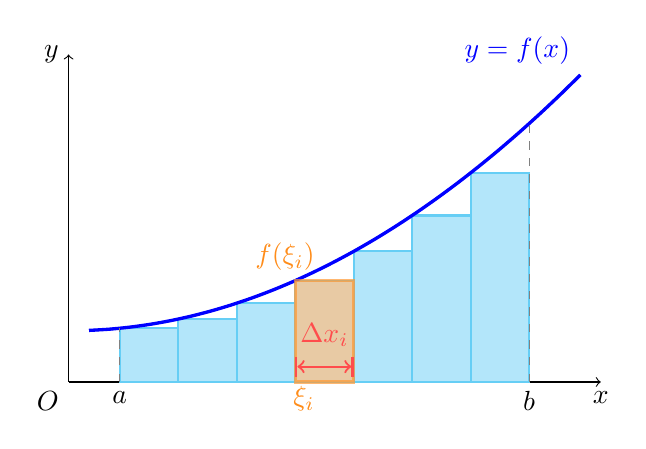
\begin{tikzpicture}[scale=1.3]
    % 定义函数和区间
    \def\a{0.5}     % 左端点
    \def\b{4.5}     % 右端点
    \def\n{7}       % 分割份数
    
    % 坐标轴（y轴上限调整为3.2）
    \draw[->] (0,0) -- (5.2,0) node[below] {$x$};
    \draw[->] (0,0) -- (0,3.2) node[left] {$y$};
    
    % 原点标签
    \node[below left] at (0,0) {$O$};
    
    % 画曲线 y = f(x) = 0.1x^2 + 0.5
    \draw[domain=0.2:5.0, smooth, thick, blue] 
        plot (\x, {0.1*\x*\x + 0.5}) 
        node[above left] {$y=f(x)$};
    
    % 计算并绘制矩形（取左端点高度）
    \foreach \i in {0,1,...,6} {
        \pgfmathsetmacro\xleft{\a + (\b-\a)*\i/\n}
        \pgfmathsetmacro\xright{\a + (\b-\a)*(\i+1)/\n}
        \pgfmathsetmacro\fheight{0.1*(\xleft)^2 + 0.5}
        
        \fill[cyan!30, draw=cyan!60, thick] 
            (\xleft, 0) rectangle (\xright, \fheight);
    }
    
    % 再画一次曲线，使其盖在矩形上面
    \draw[domain=0.2:5.0, smooth, very thick, blue] 
        plot (\x, {0.1*\x*\x + 0.5});
    
    % 区间端点竖线
    \draw[dashed, gray] (\a, 0) -- (\a, {0.1*(\a)^2 + 0.5});
    \draw[dashed, gray] (\b, 0) -- (\b, {0.1*(\b)^2 + 0.5});
    
    % 区间标记
    \node[below] at (\a, 0) {$a$};
    \node[below] at (\b, 0) {$b$};
    
    % 突出显示第5个矩形 (索引4)
    \pgfmathsetmacro\xleftfive{\a + (\b-\a)*3/\n}
    \pgfmathsetmacro\xrightfive{\a + (\b-\a)*4/\n}
    \pgfmathsetmacro\fheightfive{0.1*(\xleftfive)^2 + 0.5}
    
    \fill[orange!50, draw=orange!80, very thick, opacity=0.7] 
        (\xleftfive, 0) rectangle (\xrightfive, \fheightfive);
    
    % 标注 xi_i 和 f(xi_i)
    \pgfmathsetmacro\xmid{\xleftfive + (\xrightfive-\xleftfive)/2}
    \node[above left, orange!90] at (\xmid, \fheightfive) {$f(\xi_i)$};
    \node[below left, orange!90] at (\xmid, 0.05) {$\xi_i$};
    
    % 宽度标注
    \draw[|<->|, red!70, thick] 
        (\xleftfive, 0.15) -- (\xrightfive, 0.15);
    \node[above, red!70] at (\xmid, 0.25) {$\Delta x_i$};
    
\end{tikzpicture}
\end{center}

那要怎么求这个曲边梯形的面积呢？我们可以把区间 $[a, b]$ 分成 $n$ 个小段，每段宽度为 $\Delta x_i$，在每段上取一个点 $\xi_i$，用 $f(\xi_i) \cdot \Delta x_i$ 作为这一小条矩形的面积。那么所有小矩形面积之和就是：
\[
\sum_{i=1}^{n} f(\xi_i)\, \Delta x_i
\]

当$n$足够大的时候，曲线就可以近似看成直线，面积就可以用小矩形近似，也就是说，我们把区间$[a, b]$分得越细，近似就越精确。用数学语言表示就是：当$n \to \infty$，$\Delta x_i \to 0$时：
\[
\int_a^b f(x)\, dx = \lim_{\Delta x_i \to 0} \sum_{i=1}^{n} f(\xi_i)\, \Delta x_i
\]

由此，我们得出了定积分的定义：

\begin{definition}{定积分}{}
设函数 \(f(x)\) 在 \([a,b]\) 上有界，在 \([a,b]\) 中任意插入若干个分点
\[
a=x_0<x_1<x_2<\cdots<x_n=b
\]
把区间 \([a,b]\) 分成 \(n\) 个小区间
\[
[x_0,x_1], \ [x_1,x_2], \ \cdots, \ [x_{n-1},x_n]
\]
各个小区间的长度依次为
\[
\Delta x_1=x_1-x_0, \ \Delta x_2=x_2-x_1, \ \cdots, \ \Delta x_n=x_n-x_{n-1}
\]
在每个小区间 \([x_{i-1},x_i]\) 上任取一点 \(\xi_i\) (\(x_{i-1} \leqslant \xi_i \leqslant x_i\))，作函数值 \(f(\xi_i)\) 与小区间长度 \(\Delta x_i\) 的乘积 \(f(\xi_i) \cdot \Delta x_i\)，并作出和

\[
S=\sum_{i=1}^{n} f(\xi_i) \Delta x_i
\]

记 \(\lambda = \max\{\Delta x_1, \Delta x_2, \cdots, \Delta x_n\}\)，如果当 \(\lambda \to 0\) 时，\(S\) 的极限总存在，且与闭区间 \([a,b]\) 的分法及点 \(\xi_i\) 的取法无关，那么我们就说\(f(x)\)在\([a,b]\)上\textbf{可积}，并且称这个极限 \(I\) 为函数 \(f(x)\) 在区间 \([a,b]\) 上的定积分，记作 \(\int_{a}^{b} f(x) dx\)，即：

\[
\int_{a}^{b} f(x) dx = \lim_{\lambda \to 0} \sum_{i=1}^{n} f(\xi_i) \Delta x_i = I
\]

其中 \(f(x)\) 称为\textbf{被积函数}，\(f(x) dx\) 称为\textbf{被积表达式}，\(x\) 称为\textbf{积分变量}，\(a\) 称为\textbf{积分下限}，\(b\) 称为\textbf{积分上限}，\([a,b]\) 称为\textbf{积分区间}。

\end{definition}

定积分定义的背后蕴含着“以直代曲”和“微元法”朴素的数学思想。这也说明了积分号 $\int$ 的来源：$\int$是一个拉长的字母 S（Sum），代表求和。

这个定义看上去很复杂，其实说的就是一件事：分割，近似，求和，取极限。把区间分割成一个个小区间，在小区间里用小矩形近似小曲边梯形，把所有小矩形的面积加起来，再让小区间长度趋近于$0$，取和的极限，定积分本质上说的就是这么一回事。

而几何意义就更直观了。$\int_{a}^{b} f(x) dx$表示由曲线$f(x)$、$x$ 轴以及两条竖直线 $x = a$ 和 $x = b$ 围成的区域的面积。

但要注意，如果 $f(x)$ 在某些地方为负，那“面积”怎么算？定积分对负的部分会给出负值，因为 $\int_a^b f(x)\, dx$ 计算的是\textbf{代数面积}，也就是说，$x$ 轴上方的面积为正，下方的面积为负，最后再加在一起。

根据定义，我们能得到几个性质：

\begin{theorem}{初等函数的可积性}{}
  任何初等函数在其定义域内的任意闭区间上都是可积的。
\end{theorem}

\begin{theorem}{零区间积分}{}
  \[\int_{a}^{a} f(x) dx=0\]
\end{theorem}

\begin{theorem}{线性性质}{} 
  若$f,g$可积，$\alpha,\beta \in \mathbb{R}$，则$\alpha f+\beta g$可积，且：

  \[\int_{a}^{b} [\alpha f(x)+\beta g(x)] dx=\alpha \int_{a}^{b} f(x) dx+\beta \int_{a}^{b} g(x) dx\]
\end{theorem}

\begin{theorem}{上下限互换}{}
  \[\int_{a}^{b} f(x) dx=-\int_{b}^{a} f(x) dx\]
\end{theorem}

\begin{theorem}{区间长度性质}{}
  \[\int_{a}^{b} dx=b-a\]
\end{theorem}


由此得到：

\begin{theorem}{区间可加性}{} 
  对任意$a,b,c\in \mathbb{R} $，有：

  \[\int_{a}^{b} f(x) dx=\int_{a}^{c} f(x) dx+\int_{c}^{b} f(x) dx\]
\end{theorem}

\begin{theorem}{奇偶性}{} 
  设$f(x)$在区间$[-a,a]$上可积。

  若$f(x)$为奇函数，则：\(\int_{-a}^{a} f(x) dx=0\)

  若$f(x)$为偶函数，则：\(\int_{-a}^{a} f(x) dx=2\int_{0}^{a} f(x) dx\)
\end{theorem}

\begin{theorem}{保序性}{} 
  若$f(x)\leq g(x)$，则：
  \[\int_{a}^{b} f(x) dx \leq \int_{a}^{b} g(x) dx\]
\end{theorem}

我们来看几个例子：

\begin{myexample}
  用定积分的几何意义，求 $\int_0^1 x\, dx$。

  $\int_0^1 x\, dx$表示由直线$y=x$、$x$ 轴以及两条竖直线 $x = 0$ 和 $x = 1$ 围成的区域的面积。

  直观上，$f(x) = x$ 在 $[0, 1]$ 上是一条从原点出发到 $(1, 1)$ 的直线，曲边梯形退化为一个直角三角形，底为 $1$，高为 $1$，面积为 $\frac{1}{2}$。

  因此 $\int_0^1 x\, dx = \frac{1}{2}$。
\end{myexample}

\begin{myexample}
  用定积分的几何意义，求 $\int_0^{2\pi} \sin x\, dx$。

  $\int_0^{2\pi} \sin x\, dx$表示由曲线$y=\sin x$、$x$ 轴以及两条竖直线 $x = 0$ 和 $x = 2\pi$ 围成的区域的面积。

  直观上，$\sin x$ 在 $[0, \pi]$ 上为正，在 $[\pi, 2\pi]$ 上为负。两个区域的几何形状完全对称，面积相等但符号相反，所以代数面积为 $0$。
\end{myexample}

某种程度上，这也算是定积分奇偶性的体现。

如果要求实际的面积，那就需要把负的部分取绝对值，分段积分，也就是：\(\int_a^b |f(x)|\, dx\)

在上面的例子中，$\sin x$ 在 $[0, 2\pi]$ 上的实际面积为 $\int_0^\pi \sin x\, dx + \int_\pi^{2\pi} (-\sin x)\, dx$，即一上一下的面积之和。

总结一下：

定积分 $\int_a^b f(x)\, dx$ 的几何意义是代数面积。如果 $f(x) \geq 0$，那它就是普通的面积。如果要求实际面积，需要取绝对值分段积分。

定积分的定义是分割，近似，求和，取极限。


\subsection{积分上限函数}

我们已经知道定积分 $\int_a^b f(x)\,dx$ 表示的是曲边梯形的面积。但如果我们把上限 $b$ 换成一个变量 $x$，情况就变了。$\int_a^x f(t)\,dt$ 不再是一个固定的数，而是随着 $x$ 的变化而变化。当 $x$ 变大时，积分区间变长，面积就变大。$x$ 变小时，面积就变小。也就是说，这个时候 $\int_a^x f(t)\,dt$ 是一个关于 $x$ 的函数。

这里要注意我们的积分变量用 $t$ 而不用 $x$，这是为了避免和积分上限 $x$ 混淆。

由此我们有：

\begin{definition}{积分上限函数}{}
设 $f(x)$ 在 $[a, b]$ 上可积，则对任意 $x \in [a, b]$，定义
\[
\Phi(x) = \int_a^x f(t)\, dt
\]
$\Phi(x)$ 称为 $f(x)$ 在 $[a, b]$ 上的\textbf{积分上限函数}。
\end{definition}

这个函数有一个极其重要的性质：它对 $x$ 的导数恰好就是被积函数 $f(x)$。

\begin{theorem}{积分上限函数的性质}{}
设 $f(x)$ 在 $[a, b]$ 上连续，则 $\Phi(x) = \int_a^x f(t)\, dt$ 在 $[a, b]$ 上可导，且
\[
\Phi'(x) = \frac{d}{dx} (\int_a^x f(t)\, dt) = f(x)
\]
\end{theorem}

我们简单证明一下：

证明它，我们需要分为三步。第一步，先证明估值定理：

根据连续函数的最值定理：若 $f(x)$ 在闭区间 $[a,b]$ 上连续，则 $f(x)$ 在 $[a,b]$ 上一定能取到最大值和最小值。记最大值为$M$，最小值为$m$，则有：\[m\leq f(x)\leq M\]

由区间长度性质得到：\(\int_{a}^{b} m dx=m(b-a)\)，\(\int_{a}^{b} M dx=M(b-a)\)

由保序性：\[m(b-a)\leq \int_{a}^{b} f(x) dx\leq M(b-a)\]

于是我们证明了估值定理。它给出了曲边梯形面积的上下界估计：

\begin{theorem}{估值定理}{}
设 $f(x)$ 在 $[a, b]$ 上连续且可积，且$\exists m,M\in \mathbb{R} $，使得$m\leq f(x)\leq M$，则有：
\[
m(b-a)\leq \int_{a}^{b} f(x) \,dx \leq M(b-a)
\]
\end{theorem}

第二步，证明积分中值定理：

由估值定理：\(m(b-a)\leq \int_{a}^{b} f(x) dx\leq M(b-a)\)，两边除以$b-a$，得到：\[
m\leq \frac{1}{b-a} \int_{a}^{b} f(x) \,dx \leq M
\]

记$\mu =\frac{1}{b-a} \int_{a}^{b} f(x) \,dx$，则$\mu$的大小介于$m$与$M$之间。

由于$f(x)$连续，不妨设$f(c)=m$，$f(d)=M$，其中$c,d\in[a,b]$，且$c<d$。

由连续函数的介值定理：若 $f(x)$ 在闭区间 $[c,d]$ 上连续，且 $f(c) \neq f(d)$，则对于 $f(c)$ 与 $f(d)$ 之间的任意一个数 $\mu$，都存在至少一个 $\xi \in (c,d)$，使得 $f(\xi) = \mu$。

则有：\[\int_{a}^{b} f(x) \,dx =f(\xi )(b-a)\]

于是我们证明了积分中值定理。它在微积分中有重要地位：

\begin{theorem}{积分中值定理}{}
设 $f(x)$ 在 $[a, b]$ 上连续且可积，则$\exists \xi \in [a,b]$，使得：
\[\int_{a}^{b} f(x) \,dx =f(\xi )(b-a)\]
\end{theorem}

第三步，证明积分上限函数的性质：

由区间可加性与上下限互换：\[\Phi (x+h)-\Phi (x)=\int_a^{x+h} f(t)\, dt-\int_a^x f(t)\, dt=\int_x^{x+h} f(t)\, dt\]

其中$h>0$且$x+h\in [a,b]$。

由积分中值定理：\(\int_x^{x+h} f(t)\, dt =h \cdot f(\xi )\)，两边除以$h$，即：\(\frac{1}{h} \int_x^{x+h} f(t)\, dt =f(\xi )\)

其中$\xi \in [x,x+h]$，所以$0\leq \xi -x\leq h$。

令$h\rightarrow 0$，由夹逼定理：$\lim_{h \to 0} (\xi -x) = 0 $，则$\lim_{h \to 0} \xi = x $。由于$f(x)$连续，因此$\lim_{h \to 0} f(\xi) = f(x) $。

综上，我们得到：

\[\Phi '(x)=\lim_{h \to 0}  \frac{\Phi (x+h)-\Phi (x)}{h} =\lim_{h \to 0} f(\xi)=f(x)\]

证毕。

这个性质还可以进一步推广：如果积分上限不是 $x$ ，而是一个关于 $x$ 的函数 $u(x)$，则需要加上链式法则：

\[
\Phi '(x)=\frac{d}{dx} (\int_a^{u(x)} f(t)\, dt) = f(u(x)) \cdot u'(x)
\]


我们举例说明一下。

\begin{myexample}
  设 $\Phi(x) = \int_0^x t^2\, dt$，求 $\Phi'(x)$。

  被积函数 $f(t) = t^2$，积分上限是 $x$，所以：
  \[
  \Phi'(x) = \frac{d}{dx} (\int_0^x t^2\, dt) = x^2
  \]
\end{myexample}

\begin{myexample}
  设 $\Phi(x) = \int_1^x \frac{\sin t}{t}\, dt$，求 $\Phi'(x)$。

  被积函数 $f(t) = \frac{\sin t}{t}$，积分上限是 $x$，所以：
  \[
  \Phi'(x) = \frac{\sin x}{x}
  \]

\end{myexample}

  $\int_{}^{} \frac{\sin t}{t} \,dt $ 是无法用初等函数表达的，但积分上限函数的导数仍然可以直接写出。这就是这个性质的强大之处，即使你不会算积分，也能求导。

\begin{myexample}
  求 $\frac{d}{dx} (\int_0^{x^2} \sin t\, dt)$。

  令 $u(x) = x^2$，则被积函数在 $t = x^2$ 处取值，再乘以 $u'(x) = 2x$：
  \[
  \frac{d}{dx} (\int_0^{x^2} \sin t\, dt) = \sin x^2 \cdot 2x = 2x\sin x^2
  \]
\end{myexample}

积分上限函数的导数公式是连接不定积分和定积分的桥梁，也是接下来微积分基本定理的基石。没有这个公式，我们就没有办法把“求面积”和“求原函数”联系起来。


\subsection{微积分基本定理}

前面我们学了不定积分，接下来我们学习著名的微积分基本定理，这个定理将揭示不定积分与定积分的内在联系，也是整个微积分学中最核心、最深刻的定理。

\begin{theorem}{微积分基本定理}{}
设 $f(x)$ 在 $[a, b]$ 上连续，$F(x)$ 是 $f(x)$ 在 $[a, b]$ 上的任意一个原函数，则：
\[
\int_a^b f(x)\, dx = F(b) - F(a)
\]
\end{theorem}

有时为了书写方便，也记作\(\int_a^b f(x)\, dx = [F(x)]_a^b\)。

这个定理也被称为牛顿-莱布尼茨公式，因为牛顿和莱布尼茨各自独立地发明了微积分，并分别从不同角度揭示了微分与积分之间的互逆关系。他们的贡献共同奠定了微积分的基础。

为什么这个定理成立？我们简要证明一下：

我们已经证明了积分上限函数 $\Phi(x) = \int_a^x f(t)\,dt$ 满足 $\Phi'(x) = f(x)$，所以 $\Phi(x)$ 本身就是 $f(x)$ 的一个原函数。那么 $\Phi(x)$ 和 $F(x)$ 只差一个常数 $C$，也就是：

\[F(x) = \Phi(x) + C\]

令 $x = a$，得： \[F(a)=\Phi(a) +C = \int_a^a f(t)\,dt + C \]

由零区间积分，得\(\int_a^a f(t)\,dt=0\)，即$C = F(a)$。

同理，令 $x = b$，得：
\[
F(b)=\Phi(b) +C = \int_a^b f(t)\,dt + C
\]

代入$C = F(a)$，移项得：

\[
\int_a^b f(t)\,dt=F(b)-F(a)
\]

证毕。

这个定理告诉我们，\textbf{定积分等于原函数在上限和下限处的值之差}。它把“求面积”转化成了“求原函数再代值”，也就是把一个几何问题转化为了代数问题。之前我们求 $\int_0^1 x\,dx$ 靠的是几何直觉，现在有了这个定理，我们可以用代数方法算出结果：

\begin{myexample}
  求 $\int_0^1 x\, dx$。

  $x$ 的一个原函数是 $\frac{x^2}{2}$，所以：
  
  \[
  \int_0^1 x\, dx= \frac{1^2}{2} - \frac{0^2}{2} = \frac{1}{2}
  \]
\end{myexample}

\begin{myexample}
  求 $\int_0^\pi \sin x\, dx$。

  $\sin x$ 的一个原函数是 $-\cos x$，所以：
  \[
  \int_0^\pi \sin x\, dx = (-\cos\pi) - (-\cos 0) = 1 - (-1) = 2
  \]
\end{myexample}

几何上，这正是 $\sin x$ 在 $[0, \pi]$ 上的面积。

\begin{myexample}
  求 $\int_1^e \frac{1}{x}\, dx$。

  $\frac{1}{x}$ 的一个原函数是 $\ln|x|$，所以：
  \[
  \int_1^e \frac{1}{x}\, dx = \ln e - \ln 1 = 1 - 0 = 1
  \]
\end{myexample}

\begin{myexample}
  求 $\int_0^1 e^x\, dx$。

  $e^x$ 的一个原函数是 $e^x$，所以：
  \[
  \int_0^1 e^x\, dx = e^1 - e^0 = e - 1
  \]
\end{myexample}

需要注意的是，使用牛顿-莱布尼茨公式时，$f(x)$ 必须在 $[a, b]$ 上连续。如果 $f(x)$ 在区间内有间断点，直接套公式可能出错。不连续的函数，我们可以分段求定积分，再将结果相加。

形象地说，积分是在总结过去，微分是在展望未来。积分从堆积的过往还原完整的面积，微分从当下的斜率预见未来的趋势。积分把一个个音符变成一首完整的歌，微分把一首歌分解为一个个音符。

微积分基本定理是整个微积分的枢纽。正如牛顿和莱布尼茨各自独立发现的那样，它把微分学和积分学统一了起来。

它是一座连接微分和积分的桥梁。牛顿用它描述了天体的运行，莱布尼茨用它书写了自然的规律。

这正是牛顿-莱布尼茨公式所告诉我们的。

那座桥梁，就是枢纽本身。

\subsection{定积分的计算方法}

有了微积分基本定理，定积分的计算就变成了“找原函数、代上限、减下限”的公式化操作。因此我们前面学过的所有不定积分技巧都可以直接用在定积分上。只不过有一些细节上的区别。

不定积分的换元法用 $u$ 替换后要把 $x$ 代回去。但定积分不需要代回去。换元的同时把积分上下限也换掉，最后直接用新变量的上下限代值计算。

\begin{theorem}{定积分的换元法}{}
设 $f(x)$ 在 $[a, b]$ 上连续，$x = \phi(t)$ 在 $[\alpha, \beta]$ 上单调可微，且 $\phi(\alpha) = a$，$\phi(\beta) = b$，则：
\[
\int_a^b f(x)\, dx = \int_\alpha^\beta f(\phi(t)) \cdot \phi'(t)\, dt
\]
\end{theorem}

也就是说，换元之后的上下限不一样了，因此，\textbf{换元时上下限要跟着换}。$\phi(\alpha) = a$ 意味着新下限 $\alpha$ 对应旧下限 $a$，$\phi(\beta) = b$意味着新上限 $\beta$ 对应旧上限 $b$。如果用 $u$ 代换，也是完全一样的，$u$ 的上下限由 $x$ 的上下限决定。

我们来看几个例子：

\begin{myexample}
  求 $\int_0^4 \frac{1}{1+\sqrt{x}}\, dx$。

  令 $t = \sqrt{x}$，则 $x = t^2$，$dx = 2t\, dt$。换上下限：$x = 0$ 时 $t = 0$，$x = 4$ 时 $t = 2$。
  \[
  \int_0^4 \frac{1}{1+\sqrt{x}}\, dx = \int_0^2 \frac{1}{1+t} \cdot 2t\, dt = \int_0^2 \frac{2t}{1+t}\, dt
  \]

  所以：
  \[
  \int_0^2 \frac{2t}{1+t}\, dt = [2t - 2\ln|1+t|]_0^2 = (4 - 2\ln 3) - (0 - 0) = 4 - 2\ln 3
  \]
\end{myexample}

这个例子说明，最后代入的是新变量 $t$ 的上下限 $0$ 和 $2$，不需要代回 $x$。

\begin{myexample}
  求 $\int_0^1 \sqrt{1-x^2}\, dx$。

  令 $x = \sin t$，则 $dx = \cos t\, dt$，$\sqrt{1-x^2} = \cos t$。换上下限：$x = 0$ 时 $t = 0$，$x = 1$ 时 $t = \frac{\pi}{2}$。
  \[
  \int_0^1 \sqrt{1-x^2}\, dx = \int_0^{\frac{\pi}{2}} \cos t \cdot \cos t\, dt = \int_0^{\frac{\pi}{2}} \cos^2 t\, dt
  \]

  用降幂公式 $\cos^2 t = \frac{1+\cos 2t}{2}$，得：
  \[
  \int_0^{\frac{\pi}{2}} \frac{1+\cos 2t}{2}\, dt = \frac{1}{2}[t + \frac{\sin 2t}{2}]_0^{\frac{\pi}{2}} = \frac{1}{2}(\frac{\pi}{2} + 0) - 0 = \frac{\pi}{4}
  \]
\end{myexample}
  
  几何上，这正是单位圆在第一象限的面积，大小正是$\frac{\pi}{4}$，完全合理。

和换元法一样，分部积分法也可以直接用在定积分上，只是公式里多了上下限：

\begin{theorem}{定积分的分部积分法}{}
\[
\int_a^b u\, dv = [uv]_a^b - \int_a^b v\, du
\]
\end{theorem}

\begin{myexample}
  求 $\int_0^1 x e^x\, dx$。

  令 $u = x$，$dv = e^x\, dx$，则 $du = dx$，$v = e^x$。代入公式：
  \[
  \int_0^1 x e^x\, dx = [xe^x]_0^1 - \int_0^1 e^x\, dx = (1 \cdot e - 0) - [e^x]_0^1 = e - (e - 1) = 1
  \]
\end{myexample}

\begin{myexample}
  求 $\int_0^{\frac{\pi}{2}} x \cos x\, dx$。

  令 $u = x$，$dv = \cos x\, dx$，则 $du = dx$，$v = \sin x$。代入公式：
  \[
  \int_0^{\frac{\pi}{2}} x \cos x\, dx = [x\sin x]_0^{\frac{\pi}{2}} - \int_0^{\frac{\pi}{2}} \sin x\, dx = \frac{\pi}{2} \cdot 1 - 0 - [-\cos x]_0^{\frac{\pi}{2}} = \frac{\pi}{2} - (0 - (-1)) = \frac{\pi}{2} - 1
  \]
\end{myexample}

总结一下：

定积分的计算方法和不定积分完全一致，区别只有两点，换元时上下限跟着变，计算结果直接用新变量的上下限代值计算。

\subsection{反常积分}

到目前为止，我们讨论的定积分都有两个隐含的前提：积分区间是有限的，被积函数是有界的。但实际中常常遇到不满足这两个条件的情形。比如积分区间是无穷的，例如$\int_1^{+\infty} \frac{1}{x^2}\,dx$，或者被积函数在某点无界，例如$\int_0^1 \frac{1}{\sqrt{x}}\,dx$。这类积分我们统一叫做\textbf{反常积分}。

反常积分的计算思路很简单：先用有限区间上的定积分来近似，再取极限。

\begin{definition}{无穷区间上的反常积分}{}
设 $f(x)$ 在 $[a, +\infty)$ 上连续，若极限
\[
\lim_{b \to +\infty} \int_a^b f(x)\, dx
\]
存在，则称反常积分 $\int_a^{+\infty} f(x)\, dx$ \textbf{收敛}，并定义$\int_a^{+\infty} f(x)\, dx$的值为该极限。若极限不存在，则称该反常积分\textbf{发散}。
\end{definition}

类似地可以定义 $\int_{-\infty}^b f(x)\,dx$ 和 $\int_{-\infty}^{+\infty} f(x)\,dx$。后者的计算要拆成两段：
\[
\int_{-\infty}^{+\infty} f(x)\, dx = \int_{-\infty}^{0} f(x)\, dx + \int_0^{+\infty} f(x)\, dx
\]

当两段都收敛时才说整个积分收敛。

\begin{myexample}
  判断 $\int_1^{+\infty} \frac{1}{x^2}\, dx$ 是否收敛，若收敛则求值。

  先算有限区间上的定积分：
  \[
  \int_1^b \frac{1}{x^2}\, dx = [-\frac{1}{x}]_1^b = -\frac{1}{b} + 1 = 1 - \frac{1}{b}
  \]

  再取极限：
  \[
  \int_1^{+\infty} \frac{1}{x^2}\, dx = \lim_{b \to +\infty} (1 - \frac{1}{b}) = 1
  \]

  因此该积分收敛，值为 $1$。
\end{myexample}

\begin{myexample}
  判断 $\int_1^{+\infty} \frac{1}{x}\, dx$ 是否收敛。

  \[
  \int_1^b \frac{1}{x}\, dx = [\ln x]_1^b = \ln b
  \]

  再取极限：
  \[\lim_{b \to +\infty} \ln b = +\infty\]
  
  极限不存在，所以积分发散。
\end{myexample}

接下来我们讨论被积函数在某点无界的情况。我们定义：

\begin{definition}{瑕点}{}
  若函数$f(x)$在$a$点的任一邻域内都无界，则称$a$为函数$f(x)$的\textbf{瑕点}。
\end{definition}

瑕点一定是间断点或函数未定义点，但间断点不一定是瑕点。

由此引出无界函数的反常积分：

\begin{definition}{无界函数的反常积分}{}
设 $f(x)$ 在 $(a, b]$ 上连续，点$a$ 为$f(x)$的瑕点，若极限
\[
\lim_{t \to a^+} \int_t^b f(x)\, dx
\]
存在，则称反常积分 $\int_a^b f(x)\, dx$ \textbf{收敛}，并定义$\int_a^b f(x)\, dx$的值为该极限。若极限不存在，则称该反常积分\textbf{发散}。
\end{definition}

类似地可以定义点$b$ 为$f(x)$的瑕点时函数 \(f(x)\) 在 \([a, b)\) 上的反常积分和点$c$ 为$f(x)$的瑕点时函数 \(f(x)\) 在 \([a, c)\) 及 \((c, b]\) 上的反常积分，这两个积分仍然记为 \(\int_a^b f(x) \, dx\)，后者的计算要拆成两段：
\[
\int_a^b f(x) \, dx = \int_a^c f(x) \, dx + \int_c^b f(x) \, dx
\]

无界函数的反常积分又称为\textbf{瑕积分}。

\begin{myexample}
  判断 $\int_0^1 \frac{1}{\sqrt{x}}\, dx$ 是否收敛。

  $x = 0$ 是瑕点。先算：
  \[
  \int_t^1 \frac{1}{\sqrt{x}}\, dx = [2\sqrt{x}]_t^1 = 2 - 2\sqrt{t}
  \]

  再取极限：
  \[
  \int_0^1 \frac{1}{\sqrt{x}}\, dx = \lim_{t \to 0^+} (2 - 2\sqrt{t}) = 2
  \]

  极限存在，收敛，值为 $2$。
\end{myexample}

\begin{myexample}
  判断 $\int_0^1 \frac{1}{x}\, dx$ 是否收敛。

  $x = 0$ 是瑕点。先算：
  \[
  \int_t^1 \frac{1}{x}\, dx = [\ln x]_t^1 = 0 - \ln t = -\ln t
  \]
  
  再取极限：
  \[
  \lim_{t \to 0^+} (-\ln t) = +\infty
  \]
  
  极限不存在，发散。
\end{myexample}

上面两个例子的瑕点都在左端点 $a$。如果瑕点在右端点 $b$，方法类似，只是极限方向不同。

\begin{myexample}
  判断 $\int_0^1 \frac{1}{\sqrt{1-x}}\, dx$ 是否收敛。

  $x = 1$ 是瑕点。按定义，先算：
  \[
  \int_0^t \frac{1}{\sqrt{1-x}}\, dx = [-2\sqrt{1-x}]_0^t = -2\sqrt{1-t} + 2
  \]

  再取极限：
  \[
  \int_0^1 \frac{1}{\sqrt{1-x}}\, dx = \lim_{t \to 1^-} (-2\sqrt{1-t} + 2) = 2
  \]

  极限存在，收敛，值为 $2$。
\end{myexample}

如果瑕点在区间内部，则需要拆成两段分别处理：

\begin{myexample}
  判断 $\int_{-1}^1 \frac{1}{x^2}\, dx$ 是否收敛。

  $x = 0$ 是瑕点，它在区间内部。拆成两段：
  \[
  \int_{-1}^1 \frac{1}{x^2}\, dx = \int_{-1}^0 \frac{1}{x^2}\, dx + \int_0^1 \frac{1}{x^2}\, dx
  \]

  分别计算。第一段，$x = 0$ 是右端瑕点：
  \[
  \int_{-1}^t \frac{1}{x^2}\, dx = [-\frac{1}{x}]_{-1}^t = -\frac{1}{t} - 1
  \]

  再取极限：
  \[\lim_{t \to 0^-} (-\frac{1}{t} - 1) = +\infty\]
  
  这个瑕积分第一段就发散了，既然有一段发散，那么整个积分就发散，不需要再算第二段。
\end{myexample}

总结一下反常积分的计算步骤：

如果是无穷区间上的积分，就把无穷上限换成有限上限 $b$，先算定积分，再令 $b \to +\infty$ 或 $b \to -\infty$ 取极限。极限存在就收敛，不存在就发散。

如果是瑕积分，瑕点在端点$a$，就把瑕点换成$t$算定积分，再令$t \to a^+$ 取极限。如果瑕点在中间，就拆成两段，分别处理。极限存在就收敛，不存在就发散。

本质上，反常积分就是“先积分，后取极限”。它把定积分的概念从有限推广到了无穷，因此所有不定积分技巧和定积分技巧都可以直接用在反常积分上。

\subsection{$\Gamma$函数}

最后介绍一个在数学中极其重要的特殊函数，$\Gamma$ 函数。它的定义是一个反常积分：

\begin{definition}{$\Gamma$函数}{}
\[
\Gamma(s) = \int_0^{+\infty} x^{s-1} e^{-x}\, dx, \quad s > 0
\]
\end{definition}

这个积分把 $s$ 从离散的自然数推广到了连续的正实数。它有一个非常漂亮的性质：

\begin{theorem}{$\Gamma$函数的递推公式}{}
\[
\Gamma(s+1) = s \cdot \Gamma(s)
\]
\end{theorem}

我们用分部积分法简要证明一下：

令 $u = x^s$，$dv = e^{-x}\,dx$，则 $du = sx^{s-1}\,dx$，$v = -e^{-x}$，则：
\[
\Gamma(s+1) = \int_0^{+\infty} x^s e^{-x}\, dx = [-x^s e^{-x}]_0^{+\infty} + s\int_0^{+\infty} x^{s-1} e^{-x}\, dx = 0 + s\,\Gamma(s)
\]

这个递推公式让我们可以算出所有正整数处的 $\Gamma$ 值。首先计算 $\Gamma(1)$：
\[
\Gamma(1) = \int_0^{+\infty} e^{-x}\, dx = [-e^{-x}]_0^{+\infty} = 0 - (-1) = 1
\]

然后由递推公式：
\[
\Gamma(2) = 1 \cdot \Gamma(1) = 1,\quad
\Gamma(3) = 2 \cdot \Gamma(2) = 2,\quad
\Gamma(4) = 3 \cdot \Gamma(3) = 6
\]

你发现它们有什么规律了吗？

一般地，对正整数 $n$有：
\[
\Gamma(n) = (n-1)!
\]

也就是说，$\Gamma$ 函数其实就是阶乘的连续版本。不过$\Gamma(n) = (n-1)!$差了一个 $1$ 的偏移。这个偏移是历史遗留问题，当初欧拉定义时就是这么写的，后来大家也就习惯了。

还有一个特殊值值得记住：
\[
\Gamma(\frac{1}{2}) = \int_0^{+\infty} x^{-\frac{1}{2}} e^{-x}\, dx = \sqrt{\pi}
\]

这个结果的证明需要用到换元 $x = t^2$ 和高斯积分 $\int_{-\infty}^{+\infty} e^{-t^2}\, dt = \sqrt{\pi}$，后者是概率论中最核心的积分之一。我们这里省略不证。

1729年，年轻的欧拉与哥德巴赫讨论一个问题：既然$n!$对所有正整数都有定义，那么对于更一般的正实数 $s$，是否也能定义一个类似的$s!$，将阶乘推广到所有正实数？后来，他在给哥德巴赫的信中，构造了 $\Gamma$ 函数的前身：

\[
\int_{0}^{1} (-\ln t)^n  \,dt 
\]

令$t = e^{-x}$，则 $dt = -e^{-x} dx$，当 $t = 0$ 时，$x \to +\infty$，当 $t = 1$ 时，$x = 0$。于是：

\[\int_{0}^{1} (-\ln t)^n  \,dt = \int_{+\infty}^{0} -x^n e^{-x} dx=\int_{0}^{+\infty} x^n e^{-x} dx\]

随后，欧拉用这个积分作为“广义阶乘”的定义。法国数学家勒让德在 1811 年首次引入了希腊字母 $\Gamma$ 来表示这个函数，并给出了现代标准定义。之后 $\Gamma$ 函数就沿用至今。

$\Gamma$ 函数在概率论、数论、物理学中都有广泛应用。它把离散的阶乘推广到了连续的实数域，将许多复杂的积分和无穷乘积转换为已知量，是连接离散数学和连续数学的一座桥梁。